\documentclass[a4paper,12pt]{article}
\usepackage{amsmath, amssymb}
\usepackage{xcolor}
\usepackage[most]{tcolorbox}
\usepackage{multicol}
\usepackage{geometry}
\usepackage{graphicx}
\usepackage{hyperref}
\graphicspath{ {../Images/} }

\geometry{left=1.5cm, right=1.5cm, top=2cm, bottom=2cm}

\title{Exercices de Nombres Complexes}
\author{}
\date{}

% Style de boîte pour les exercices
\tcbset{
    colframe=purple!70,
    colback=white,
    coltitle=black,
    fonttitle=\bfseries,
    sharp corners,
    boxrule=0.5mm,
    colbacktitle=purple!20!white,
    center title,
    boxsep=4pt,
}

% Style de boîte pour les solutions
\newtcolorbox{solutionbox}[1][]{
    colframe=green!70,
    colback=white,
    coltitle=black,
    fonttitle=\bfseries,
    sharp corners,
    boxrule=0.5mm,
    colbacktitle=green!20!white,
    title=Solution,
    boxsep=4pt,
    breakable,
    #1
}

\begin{document}

\maketitle

\begin{tcolorbox}[title=Exercice 1 - {[}Calculer{]}]
Calculer le module et l’argument des nombres complexes suivants :
\begin{enumerate}
    \item \( z = 1 + i \)
    \item \( z = 2\pi i \)
    \item \( z = 2 - 2\sqrt{3}i \)
    \item \( z = -5 - 5i \)
    \item \( z = \sqrt{6} - \sqrt{2}i \)
\end{enumerate}
\end{tcolorbox}

\begin{solutionbox}
\begin{enumerate}
    \item \( z = 1 + i \)

    \textbf{Module} :
    \[
    |z| = \sqrt{(\operatorname{Re}(z))^2 + (\operatorname{Im}(z))^2} = \sqrt{1^2 + 1^2} = \sqrt{2}
    \]

    \textbf{Argument} :
    \[
    \theta = \arctan\left(\dfrac{\operatorname{Im}(z)}{\operatorname{Re}(z)}\right) = \arctan(1) = \dfrac{\pi}{4}
    \]
    (Comme \( \operatorname{Re}(z) > 0 \) et \( \operatorname{Im}(z) > 0 \), l'argument est bien \( \dfrac{\pi}{4} \).)

    \item \( z = 2\pi i \)

    \textbf{Module} :
    \[
    |z| = \sqrt{0^2 + (2\pi)^2} = 2\pi
    \]

    \textbf{Argument} :
    \[
    \theta = \arctan\left(\dfrac{2\pi}{0}\right) = \dfrac{\pi}{2}
    \]
    (Le nombre est purement imaginaire positif.)

    \item \( z = 2 - 2\sqrt{3}i \)

    \textbf{Module} :
    \[
    |z| = \sqrt{2^2 + (-2\sqrt{3})^2} = \sqrt{4 + 12} = \sqrt{16} = 4
    \]

    \textbf{Argument} :
    \[
    \theta = \arctan\left(\dfrac{-2\sqrt{3}}{2}\right) = \arctan(-\sqrt{3}) = -\dfrac{\pi}{3}
    \]
    (Le nombre est dans le quatrième quadrant.)

    \item \( z = -5 - 5i \)

    \textbf{Module} :
    \[
    |z| = \sqrt{(-5)^2 + (-5)^2} = \sqrt{25 + 25} = \sqrt{50} = 5\sqrt{2}
    \]

    \textbf{Argument} :
    \[
    \theta = \arctan\left(\dfrac{-5}{-5}\right) = \arctan(1) = \dfrac{\pi}{4}
    \]
    Comme \( \operatorname{Re}(z) < 0 \) et \( \operatorname{Im}(z) < 0 \), l'argument est :
    \[
    \theta = \dfrac{\pi}{4} - \pi = -\dfrac{3\pi}{4}
    \]

    \item \( z = \sqrt{6} - \sqrt{2}i \)

    \textbf{Module} :
    \[
    |z| = \sqrt{(\sqrt{6})^2 + (-\sqrt{2})^2} = \sqrt{6 + 2} = \sqrt{8} = 2\sqrt{2}
    \]

    \textbf{Argument} :
    \[
    \theta = \arctan\left(\dfrac{-\sqrt{2}}{\sqrt{6}}\right) = \arctan\left(-\dfrac{1}{\sqrt{3}}\right) = -\dfrac{\pi}{6}
    \]
    (Le nombre est dans le quatrième quadrant.)
\end{enumerate}
\end{solutionbox}

\begin{tcolorbox}[title=Exercice 2 - {[}Calculer{]}]
Déterminer la forme trigonométrique et la forme exponentielle des nombres complexes suivants :
\begin{enumerate}
    \item \( z = 2 + 2i \)
    \item \( z = -3i \)
    \item \( z = 1 + \sqrt{3}i \)
    \item \( z = \dfrac{\sqrt{3}}{3} - \dfrac{1}{3}i \)
    \item \( z = -\sqrt{5} - \sqrt{5}i \)
\end{enumerate}
\end{tcolorbox}

\begin{solutionbox}
\begin{enumerate}
    \item \( z = 2 + 2i \)

    \textbf{Module} :
    \[
    |z| = \sqrt{2^2 + 2^2} = \sqrt{8} = 2\sqrt{2}
    \]

    \textbf{Argument} :
    \[
    \theta = \arctan\left(\dfrac{2}{2}\right) = \dfrac{\pi}{4}
    \]

    \textbf{Forme trigonométrique} :
    \[
    z = 2\sqrt{2} \left( \cos\left(\dfrac{\pi}{4}\right) + i\sin\left(\dfrac{\pi}{4}\right) \right)
    \]

    \textbf{Forme exponentielle} :
    \[
    z = 2\sqrt{2} \, e^{i\frac{\pi}{4}}
    \]

    \item \( z = -3i \)

    \textbf{Module} :
    \[
    |z| = |-3i| = 3
    \]

    \textbf{Argument} :
    \[
    \theta = \arctan\left(\dfrac{-3}{0}\right) = -\dfrac{\pi}{2}
    \]
    (Nombre purement imaginaire négatif.)

    \textbf{Forme trigonométrique} :
    \[
    z = 3 \left( \cos\left( -\dfrac{\pi}{2} \right) + i\sin\left( -\dfrac{\pi}{2} \right) \right)
    \]

    \textbf{Forme exponentielle} :
    \[
    z = 3\, e^{-i\frac{\pi}{2}}
    \]

    \item \( z = 1 + \sqrt{3}i \)

    \textbf{Module} :
    \[
    |z| = \sqrt{1^2 + (\sqrt{3})^2} = \sqrt{1 + 3} = 2
    \]

    \textbf{Argument} :
    \[
    \theta = \arctan\left( \dfrac{\sqrt{3}}{1} \right) = \dfrac{\pi}{3}
    \]

    \textbf{Forme trigonométrique} :
    \[
    z = 2 \left( \cos\left( \dfrac{\pi}{3} \right) + i\sin\left( \dfrac{\pi}{3} \right) \right)
    \]

    \textbf{Forme exponentielle} :
    \[
    z = 2\, e^{i\frac{\pi}{3}}
    \]

    \item \( z = \dfrac{\sqrt{3}}{3} - \dfrac{1}{3}i \)

    \textbf{Module} :
    \[
    |z| = \sqrt{\left( \dfrac{\sqrt{3}}{3} \right)^2 + \left( -\dfrac{1}{3} \right)^2} = \sqrt{ \dfrac{3}{9} + \dfrac{1}{9} } = \dfrac{2}{3}
    \]

    \textbf{Argument} :
    \[
    \theta = \arctan\left( \dfrac{ -\dfrac{1}{3} }{ \dfrac{\sqrt{3}}{3} } \right) = \arctan\left( -\dfrac{1}{\sqrt{3}} \right) = -\dfrac{\pi}{6}
    \]

    \textbf{Forme trigonométrique} :
    \[
    z = \dfrac{2}{3} \left( \cos\left( -\dfrac{\pi}{6} \right) + i\sin\left( -\dfrac{\pi}{6} \right) \right)
    \]

    \textbf{Forme exponentielle} :
    \[
    z = \dfrac{2}{3}\, e^{-i\frac{\pi}{6}}
    \]

    \item \( z = -\sqrt{5} - \sqrt{5}i \)

    \textbf{Module} :
    \[
    |z| = \sqrt{ (-\sqrt{5})^2 + (-\sqrt{5})^2 } = \sqrt{5 + 5} = \sqrt{10}
    \]

    \textbf{Argument} :
    \[
    \theta = \arctan\left( \dfrac{ -\sqrt{5} }{ -\sqrt{5} } \right) = \arctan(1) = \dfrac{\pi}{4}
    \]
    Comme les deux parties sont négatives, l'argument est :
    \[
    \theta = \dfrac{\pi}{4} - \pi = -\dfrac{3\pi}{4}
    \]

    \textbf{Forme trigonométrique} :
    \[
    z = \sqrt{10} \left( \cos\left( -\dfrac{3\pi}{4} \right) + i\sin\left( -\dfrac{3\pi}{4} \right) \right)
    \]

    \textbf{Forme exponentielle} :
    \[
    z = \sqrt{10}\, e^{-i\frac{3\pi}{4}}
    \]
\end{enumerate}
\end{solutionbox}

\begin{tcolorbox}[title=Exercice 3 - {[}Calculer{]}]
Déterminer la forme algébrique de :
\[
(-1 + i)^{13}.
\]
\end{tcolorbox}

\begin{solutionbox}
Tout d'abord, exprimons \( -1 + i \) en forme exponentielle.

\textbf{Module} :
\[
|z| = \sqrt{(-1)^2 + 1^2} = \sqrt{1 + 1} = \sqrt{2}
\]

\textbf{Argument} :
\[
\theta = \arctan\left( \dfrac{1}{-1} \right) = \arctan(-1) = -\dfrac{\pi}{4}
\]
Comme \( \operatorname{Re}(z) = -1 \) et \( \operatorname{Im}(z) = 1 \), \( z \) est dans le deuxième quadrant, donc l'argument principal est :
\[
\theta = \pi - \dfrac{\pi}{4} = \dfrac{3\pi}{4}
\]

\textbf{Forme exponentielle} :
\[
z = \sqrt{2}\, e^{i\frac{3\pi}{4}}
\]

Calculons \( z^{13} \) :
\[
z^{13} = \left( \sqrt{2}\, e^{i\frac{3\pi}{4}} \right)^{13} = (\sqrt{2})^{13} \, e^{i\frac{39\pi}{4}}
\]

Simplifions l'argument :
\[
\frac{39\pi}{4} = 9\pi + \dfrac{3\pi}{4} = 9\pi + \dfrac{3\pi}{4}
\]
Comme \( e^{i(2\pi k)} = 1 \), on peut soustraire des multiples de \( 2\pi \) :
\[
\frac{39\pi}{4} - 9\pi = \dfrac{39\pi - 36\pi}{4} = \dfrac{3\pi}{4}
\]

Donc :
\[
z^{13} = (\sqrt{2})^{13} \, e^{i\frac{3\pi}{4}}
\]

Calculons \( (\sqrt{2})^{13} \) :
\[
(\sqrt{2})^{13} = (2)^{13/2} = 2^{6.5} = 2^{6} \times \sqrt{2} = 64 \times \sqrt{2}
\]

Donc :
\[
z^{13} = 64 \sqrt{2} \, e^{i\frac{3\pi}{4}}
\]

Repassons en forme algébrique :
\[
z^{13} = 64 \sqrt{2} \left( \cos\left( \dfrac{3\pi}{4} \right) + i\sin\left( \dfrac{3\pi}{4} \right) \right)
\]

Sachant que :
\[
\cos\left( \dfrac{3\pi}{4} \right) = -\dfrac{\sqrt{2}}{2}, \quad \sin\left( \dfrac{3\pi}{4} \right) = \dfrac{\sqrt{2}}{2}
\]

Donc :
\[
z^{13} = 64 \sqrt{2} \left( -\dfrac{\sqrt{2}}{2} + i\dfrac{\sqrt{2}}{2} \right) = 64 \sqrt{2} \left( -\dfrac{\sqrt{2}}{2} + i\dfrac{\sqrt{2}}{2} \right)
\]

Simplifions :
\[
-\dfrac{\sqrt{2} \times \sqrt{2}}{2} = -\dfrac{2}{2} = -1
\]
\[
\dfrac{\sqrt{2} \times \sqrt{2}}{2} = \dfrac{2}{2} = 1
\]

Donc :
\[
z^{13} = 64 (-1 + i)
\]
\end{solutionbox}

\begin{tcolorbox}[title=Exercice 4 - {[}Calculer{]}]
Déterminer la forme exponentielle de :
\[
e^{i\frac{\pi}{4}} + e^{i\frac{\pi}{3}}.
\]
\end{tcolorbox}

\begin{solutionbox}
Calculons la somme :
\[
e^{i\frac{\pi}{4}} + e^{i\frac{\pi}{3}}.
\]

Factorisons par \( e^{i\frac{\pi}{4}} \) :
\[
e^{i\frac{\pi}{4}} + e^{i\frac{\pi}{3}} = e^{i\frac{\pi}{4}} \left(1 + e^{i\left(\frac{\pi}{3} - \frac{\pi}{4}\right)}\right).
\]

Calculons la différence d'angles :
\[
\frac{\pi}{3} - \frac{\pi}{4} = \frac{4\pi - 3\pi}{12} = \frac{\pi}{12}.
\]

Donc :
\[
e^{i\frac{\pi}{4}} + e^{i\frac{\pi}{3}} = e^{i\frac{\pi}{4}} \left(1 + e^{i\frac{\pi}{12}}\right).
\]

Utilisons la formule de somme des exponentielles complexes :
\[
1 + e^{i\alpha} = 2\cos\left(\dfrac{\alpha}{2}\right)e^{i\frac{\alpha}{2}}.
\]

Pour \( \alpha = \dfrac{\pi}{12} \) :
\[
1 + e^{i\frac{\pi}{12}} = 2\cos\left(\dfrac{\pi}{24}\right)e^{i\frac{\pi}{24}}.
\]

Ainsi :
\[
e^{i\frac{\pi}{4}} + e^{i\frac{\pi}{3}} = e^{i\frac{\pi}{4}} \times 2\cos\left(\dfrac{\pi}{24}\right) e^{i\frac{\pi}{24}} = 2\cos\left(\dfrac{\pi}{24}\right) e^{i\left(\frac{\pi}{4} + \frac{\pi}{24}\right)}.
\]

Simplifions l'argument :
\[
\frac{\pi}{4} + \frac{\pi}{24} = \frac{6\pi + \pi}{24} = \frac{7\pi}{24}.
\]

Donc la forme exponentielle cherchée est :
\[
e^{i\frac{\pi}{4}} + e^{i\frac{\pi}{3}} = 2\cos\left(\dfrac{\pi}{24}\right) e^{i\frac{7\pi}{24}}.
\]

\textbf{Conclusion} : La forme exponentielle de \( e^{i\frac{\pi}{4}} + e^{i\frac{\pi}{3}} \) est
\[
2\cos\left(\dfrac{\pi}{24}\right) e^{i\frac{7\pi}{24}}.
\]
\end{solutionbox}

\begin{tcolorbox}[title=Exercice 5 - {[}Calculer{]}]
Calculer
\[
\int_{\frac{2\pi}{3}}^{0} \cos^3(t) \, dt.
\]
\end{tcolorbox}

\begin{solutionbox}
Utilisons les expressions exponentielles des fonctions trigonométriques :
\[
\cos t = \dfrac{e^{it} + e^{-it}}{2}.
\]

Donc :
\[
\cos^3 t = \left( \dfrac{e^{it} + e^{-it}}{2} \right)^3 = \dfrac{1}{8} \left( e^{it} + e^{-it} \right)^3.
\]

Développons :
\[
\left( e^{it} + e^{-it} \right)^3 = e^{3it} + 3e^{it} + 3e^{-it} + e^{-3it}.
\]

Ainsi :
\[
\cos^3 t = \dfrac{1}{8} \left( e^{3it} + 3e^{it} + 3e^{-it} + e^{-3it} \right).
\]

Regroupons en utilisant les identités :
\[
e^{a} + e^{-a} = 2\cosh(a), \quad \text{mais ici } a \text{ est imaginaire pur}, \quad e^{ia} + e^{-ia} = 2\cos(a).
\]

Donc :
\[
\cos^3 t = \dfrac{1}{8} \left( 2\cos(3t) + 6\cos(t) \right) = \dfrac{1}{4} \cos(3t) + \dfrac{3}{4} \cos t.
\]

Ainsi, l'intégrale devient :
\[
\int_{\frac{2\pi}{3}}^{0} \cos^3 t \, dt = \dfrac{1}{4} \int_{\frac{2\pi}{3}}^{0} \cos(3t) \, dt + \dfrac{3}{4} \int_{\frac{2\pi}{3}}^{0} \cos t \, dt.
\]

Calculons les intégrales :
\[
\int \cos(3t) \, dt = \dfrac{1}{3} \sin(3t) + C, \quad \int \cos t \, dt = \sin t + C.
\]

En appliquant les bornes :
\begin{align*}
\int_{\frac{2\pi}{3}}^{0} \cos^3 t \, dt &= \dfrac{1}{4} \left[ \dfrac{1}{3} \sin(3t) \right]_{\frac{2\pi}{3}}^{0} + \dfrac{3}{4} \left[ \sin t \right]_{\frac{2\pi}{3}}^{0} \\
&= \dfrac{1}{4} \left( \dfrac{1}{3} \sin(0) - \dfrac{1}{3} \sin\left( 3 \times \dfrac{2\pi}{3} \right) \right) + \dfrac{3}{4} \left( \sin 0 - \sin \dfrac{2\pi}{3} \right).
\end{align*}

Calculons les valeurs numériques :
\[
\sin(0) = 0, \quad \sin\left( 2\pi \right) = 0, \quad \sin\left( \dfrac{2\pi}{3} \right) = \dfrac{\sqrt{3}}{2}.
\]

Ainsi :
\begin{align*}
\int_{\frac{2\pi}{3}}^{0} \cos^3 t \, dt &= \dfrac{1}{4} \left( 0 - \dfrac{1}{3} \times 0 \right) + \dfrac{3}{4} \left( 0 - \dfrac{\sqrt{3}}{2} \right) \\
&= 0 + \dfrac{3}{4} \left( -\dfrac{\sqrt{3}}{2} \right) \\
&= -\dfrac{3\sqrt{3}}{8}.
\end{align*}

\textbf{Conclusion} : La valeur de l'intégrale est \( -\dfrac{3\sqrt{3}}{8} \).
\end{solutionbox}

\begin{tcolorbox}[title=Exercice 6 - {[}Calculer{]}]
Calculer
\[
\int_{\frac{\pi}{4}}^{0} \cos^2(t) \sin^2(t) \, dt.
\]
\end{tcolorbox}

\begin{solutionbox}
Utilisons les expressions exponentielles :
\[
\cos t = \dfrac{e^{it} + e^{-it}}{2}, \quad \sin t = \dfrac{e^{it} - e^{-it}}{2i}.
\] 

Donc :
\[
\cos^2 t = \left( \dfrac{e^{it} + e^{-it}}{2} \right)^2 = \dfrac{e^{2it} + 2 + e^{-2it}}{4},
\]
\[
\sin^2 t = \left( \dfrac{e^{it} - e^{-it}}{2i} \right)^2 = \dfrac{-e^{2it} + 2 - e^{-2it}}{4}.
\]

Ainsi, le produit :
\begin{align*}
\cos^2 t \sin^2 t &= \left( \dfrac{e^{2it} + 2 + e^{-2it}}{4} \right) \left( \dfrac{-e^{2it} + 2 - e^{-2it}}{4} \right) \\
\end{align*}

Simplifions le numérateur :
\begin{align*}
(e^{2it} + 2 + e^{-2it})(-e^{2it} + 2 - e^{-2it}) &= -e^{-4it} - e^{4it} +2.
\end{align*}


Ainsi :
$$
    \cos^2t\sin^2t = \dfrac{-2\cos(4t) + 2}{16}\\
    = \dfrac{1 - \cos(4t)}{8}
$$
\end{solutionbox}

\begin{tcolorbox}[title=Exercice 7 - {[}Calculer{]}]
À l’aide de la formule de Moivre, exprimer \( \cos(3x) \) et \( \sin(3x) \) en fonction de \( \cos(x) \) et \( \sin(x) \).
\end{tcolorbox}

\begin{solutionbox}
La formule de Moivre stipule que :
\[
\left( \cos x + i\sin x \right)^n = \cos(nx) + i\sin(nx)
\]

Pour \( n = 3 \) :
\[
\left( \cos x + i\sin x \right)^3 = \cos(3x) + i\sin(3x)
\]

Développons le membre de gauche :
\[
\left( \cos x + i\sin x \right)^3 = \cos^3 x + 3i\cos^2 x \sin x - 3\cos x \sin^2 x - i\sin^3 x
\]

Regroupons les parties réelles et imaginaires :

\textbf{Partie réelle} :
\[
\cos^3 x - 3\cos x \sin^2 x
\]

\textbf{Partie imaginaire} :
\[
3\cos^2 x \sin x - \sin^3 x
\]

Ainsi, on a :
\[
\cos(3x) = \cos^3 x - 3\cos x \sin^2 x
\]
\[
\sin(3x) = 3\cos^2 x \sin x - \sin^3 x
\]

On peut également exprimer \( \sin^2 x \) et \( \cos^2 x \) en fonction de l'autre pour simplifier davantage si nécessaire.
\end{solutionbox}

\begin{tcolorbox}[title={Exercice 8 - [Raisonner]}]
Montrer que pour tout \( z \in \mathbb{U} \), il existe \( z' \in \mathbb{U} \) tel que \( zz' = 1 \).
\end{tcolorbox}

\begin{solutionbox}
Si \( z \in \mathbb{U} \), alors \( |z| = 1 \).

Considérons \( z' = \dfrac{1}{z} \).

Comme \( |z| = 1 \), on a \( |z'| = \left| \dfrac{1}{z} \right| = \dfrac{1}{|z|} = 1 \), donc \( z' \in \mathbb{U} \).

De plus, \( zz' = z \times \dfrac{1}{z} = 1 \).

Ainsi, pour tout \( z \in \mathbb{U} \), il existe \( z' = \dfrac{1}{z} \in \mathbb{U} \) tel que \( zz' = 1 \).
\end{solutionbox}

\begin{tcolorbox}[title=Exercice 9 - {[}Calculer{]}]
Résoudre les équations suivantes dans \( \mathbb{C} \) :
\begin{enumerate}
    \item \( z^4 = -1 \)
    \item \( z^3 = i \)
\end{enumerate}
\end{tcolorbox}

\begin{solutionbox}
\begin{enumerate}
    \item Résoudre \( z^4 = -1 \)

    Écrivons \( -1 \) en forme exponentielle :
    \[
    -1 = e^{i\pi + 2k\pi i}, \quad k \in \mathbb{Z}
    \]

    Donc :
    \[
    z = \left( e^{i\pi + 2k\pi i} \right)^{\frac{1}{4}} = e^{i\left( \frac{\pi}{4} + \dfrac{k\pi}{2} \right)}, \quad k = 0, 1, 2, 3
    \]

    Les solutions sont donc :
    \[
    z_0 = e^{i\frac{\pi}{4}}, \quad z_1 = e^{i\frac{3\pi}{4}}, \quad z_2 = e^{i\frac{5\pi}{4}}, \quad z_3 = e^{i\frac{7\pi}{4}}
    \]

    \item Résoudre \( z^3 = i \)

    Écrivons \( i \) en forme exponentielle :
    \[
    i = e^{i\frac{\pi}{2} + 2k\pi i}, \quad k \in \mathbb{Z}
    \]

    Donc :
    \[
    z = \left( e^{i\left( \frac{\pi}{2} + 2k\pi \right)} \right)^{\frac{1}{3}} = e^{i\left( \dfrac{\pi}{6} + \dfrac{2k\pi}{3} \right)}, \quad k = 0, 1, 2
    \]

    Les solutions sont :
    \[
    z_0 = e^{i\frac{\pi}{6}}, \quad z_1 = e^{i\frac{\pi}{6} + \frac{2\pi}{3}}, \quad z_2 = e^{i\frac{\pi}{6} + \frac{4\pi}{3}}
    \]
\end{enumerate}
\end{solutionbox}

% Exercice 10
\begin{tcolorbox}[title=Exercice 10 - {[}Calculer{]}]
Soit \( n \geq 2 \). Résoudre l’équation suivante dans \( \mathbb{C} \) :
\[
z^n = \bar{z}.
\]
\end{tcolorbox}

\begin{solutionbox}
Soit \( z \in \mathbb{C} \) tel que \( z^n = \bar{z} \).

Écrivons \( z \) sous forme exponentielle :
\[
z = r e^{i\theta}, \quad r \geq 0, \theta \in \mathbb{R}.
\]
Alors, son conjugué est :
\[
\bar{z} = r e^{-i\theta}.
\]

L'équation devient :
\[
(z)^n = \bar{z} \quad \Rightarrow \quad (r e^{i\theta})^n = r e^{-i\theta}.
\]

Simplifions :
\[
r^n e^{in\theta} = r e^{-i\theta}.
\]

Divisons les deux membres par \( r \) (supposé non nul) :
\[
r^{n-1} e^{in\theta} = e^{-i\theta}.
\]

Égalité des modules :

Todo: disjonction de cas sur parité quand n impair $-1$ ou $1$.
\[
r^{n-1} = 1 \quad \Rightarrow \quad r = 1.
\]

Égalité des arguments :
\[
n\theta = -\theta + 2k\pi, \quad k \in \mathbb{Z}.
\]

Cela donne :
\[
n\theta + \theta = 2k\pi \quad \Rightarrow \quad (n + 1)\theta = 2k\pi.
\]

Donc :
\[
\theta = \dfrac{2k\pi}{n+1}, \quad k \in \mathbb{Z}.
\]

Comme \( \theta \) est défini modulo \( 2\pi \), les valeurs distinctes de \( \theta \) sont :
\[
\theta_k = \dfrac{2k\pi}{n+1}, \quad k = 0, 1, 2, \dots, n.
\]

Ainsi, les solutions sont :
\[
z_k = e^{i\theta_k} = e^{i\frac{2k\pi}{n+1}}, \quad k = 0, 1, 2, \dots, n.
\]

\textbf{Conclusion} : Les solutions de l'équation sont les racines \((n+1)\)-ièmes de l'unité.
\end{solutionbox}

% Exercice 11
\begin{tcolorbox}[title=Exercice 11 - {[}Calculer{]}]
Soit \( n \geq 2 \). Calculer le produit des racines \( n^{\text{e}} \) de l’unité.
\end{tcolorbox}

\begin{solutionbox}
Les racines \( n \)-ièmes de l'unité sont les nombres complexes de la forme :
\[
z_k = e^{i\frac{2k\pi}{n}}, \quad k = 0, 1, 2, \dots, n-1.
\]

Le produit de ces racines est :
\[
P = \prod_{k=0}^{n-1} z_k = \prod_{k=0}^{n-1} e^{i\frac{2k\pi}{n}} = e^{i\frac{2\pi}{n} \sum_{k=0}^{n-1} k}.
\]

Calculons la somme :
\[
\sum_{k=0}^{n-1} k = \dfrac{(n-1)n}{2}.
\]

Donc :
\[
P = e^{i\frac{2\pi}{n} \cdot \dfrac{(n-1)n}{2}} = e^{i\pi(n-1)}.
\]

Comme \( e^{i\pi(n-1)} = (-1)^{n-1} \), on obtient :
\[
P = (-1)^{n-1}.
\]

\textbf{Conclusion} : Le produit des racines \( n \)-ièmes de l'unité est \( (-1)^{n-1} \).
\end{solutionbox}

% Exercice 12
\begin{tcolorbox}[title={Exercice 12 - {[}Calculer, Chercher{]}}]
Déterminer tous les nombres complexes \( z \) tels que les points d’affixes \( z \), \( z^2 \) et \( z^4 \) soient alignés.
\end{tcolorbox}

\begin{solutionbox}
Pour que les points d'affixes \( z \), \( z^2 \) et \( z^4 \) soient alignés, il faut que les vecteurs \( \overrightarrow{z z^2} \) et \( \overrightarrow{z z^4} \) soient colinéaires.

Les vecteurs \( \overrightarrow{z z^2} \) et \( \overrightarrow{z z^4} \) sont colinéaires si, et seulement si, les nombres complexes \( z^2 - z \) et \( z^4 - z \) sont colinéaires, c'est-à-dire s'il existe un réel \( \mu \) tel que :
\[
\dfrac{z^2 - z}{z^4 - z} \in \mathbb{R}
\]
Calculons ce quotient :
\[
\dfrac{z^2 - z}{z^4 - z} = \dfrac{z(z - 1)}{z(z^3 - 1)} = \dfrac{z - 1}{z^3 - 1}
\]
Donc, la condition est que le nombre complexe :
\[
Q = \dfrac{z - 1}{z^3 - 1}
\]
soit réel.

Notons que :
\[
z^3 - 1 = (z - 1)(z^2 + z + 1)
\]
Ainsi :
\[
Q = \dfrac{z - 1}{(z - 1)(z^2 + z + 1)} = \dfrac{1}{z^2 + z + 1}
\]
Donc :
\[
Q = \dfrac{1}{z^2 + z + 1}
\]
Ainsi, \( Q \) est réel si, et seulement si, \( z^2 + z + 1 \) est réel et \( Q \in \mathbb{R} \).

Donc, il faut que \( z^2 + z + 1 \) soit réel.

\textbf{Soit \( z = x + i y \)} avec \( x, y \in \mathbb{R} \).

Calculons \( z^2 + z + 1 \) :
\[
z^2 + z + 1 = (x + i y)^2 + (x + i y) + 1
\]
Développons :
\[
(x^2 - y^2 + 2i x y) + (x + i y) + 1 = (x^2 - y^2 + x + 1) + i (2 x y + y)
\]
Pour que \( z^2 + z + 1 \) soit réel, il faut que la partie imaginaire soit nulle :
\[
2 x y + y = y (2 x + 1) = 0
\]
Deux cas possibles :

\textbf{Cas 1 :} \( y = 0 \)

Donc \( z \in \mathbb{R} \)

\textbf{Cas 2 :} \( 2 x + 1 = 0 \Rightarrow x = -\dfrac{1}{2} \)

Donc \( z = -\dfrac{1}{2} + i y \)

Alors, \( z^2 + z + 1 \) est réel.

Vérifions que \( Q \) est réel dans ce cas.

Calculons \( z^2 + z + 1 \) :

Pour \( x = -\dfrac{1}{2} \), on a :
\[
x^2 - y^2 + x + 1 = \left( \dfrac{1}{4} - y^2 \right) - \dfrac{1}{2} + 1 = \dfrac{3}{4} - y^2
\]
La partie réelle est \( \dfrac{3}{4} - y^2 \)

Comme \( z^2 + z + 1 \) est réel, et \( Q = \dfrac{1}{z^2 + z + 1} \), \( Q \) est réel si \( z = -\dfrac{1}{2} + i y \).

Ainsi, les valeurs de \( z \) pour lesquelles les points \( z \), \( z^2 \) et \( z^4 \) sont alignés sont :

- Les nombres réels \( z \) (avec \( y = 0 \)).

- Les nombres complexes \( z = -\dfrac{1}{2} + i y \), avec \( y \in \mathbb{R} \).

\textbf{Conclusion :} Les nombres complexes \( z \) tels que \( z \in \mathbb{R} \) ou \( z = -\dfrac{1}{2} + i y \) avec \( y \in \mathbb{R} \) sont tels que les points \( z \), \( z^2 \) et \( z^4 \) sont alignés.

\end{solutionbox}

% Exercice 13
\begin{tcolorbox}[title={Exercice 13 - {[}Chercher, Représenter{]}}]
Soient \( A_1, \dots, A_n \) des points du plan. Peut-on trouver \( n \) points \( B_1, \dots, B_n \) tels que \( A_1, \dots, A_n \) soient les milieux respectifs des segments \([B_1B_2]\), \([B_2B_3]\), \dots, \([B_nB_1]\) ?
\end{tcolorbox}

\begin{solutionbox}
\textbf{Énoncé du problème :}

Nous devons déterminer si, pour des points \( A_1, A_2, \dots, A_n \) donnés, il est possible de trouver des points \( B_1, B_2, \dots, B_n \) tels que :
\[
A_k = \dfrac{B_k + B_{k+1}}{2}, \quad \text{pour } k = 1, 2, \dots, n,
\]
avec \( B_{n+1} = B_1 \).

\textbf{Formalisation du système :}

Les équations peuvent être réécrites sous la forme :
\[
B_{k+1} = 2A_k - B_k, \quad \text{pour } k = 1, 2, \dots, n.
\]

Nous obtenons ainsi un système d'équations linéaires récurrentes reliant les \( B_k \).

\textbf{Résolution du système :}

Pour résoudre ce système, nous pouvons exprimer les \( B_k \) en fonction de \( B_1 \) et des \( A_k \).

\textbf{Étape 1 :} Calcul des \( B_k \) en fonction de \( B_1 \).

Pour \( k = 1 \) :
\[
B_2 = 2A_1 - B_1.
\]

Pour \( k = 2 \) :
\[
B_3 = 2A_2 - B_2 = 2A_2 - (2A_1 - B_1) = 2A_2 - 2A_1 + B_1.
\]

Pour \( k = 3 \) :
\[
B_4 = 2A_3 - B_3 = 2A_3 - [2A_2 - 2A_1 + B_1] = 2A_3 - 2A_2 + 2A_1 - B_1.
\]

En continuant ce processus, pour \( k = n \), nous obtenons :

Si \( n \) est impair :

\[
B_{n+1} = B_1 = (-1)^n B_1 + 2 \sum_{k=1}^{n} (-1)^{n-k} A_k.
\]

Si \( n \) est pair :

\[
B_1 = (-1)^n B_1 + 2 \sum_{k=1}^{n} (-1)^{n-k} A_k.
\]

\textbf{Cas où \( n \) est impair :}

Pour \( n \) impair, \( (-1)^n = -1 \). L'équation devient :
\[
B_1 = -B_1 + 2 \sum_{k=1}^{n} (-1)^{n-k} A_k.
\]

En regroupant les termes en \( B_1 \) :
\[
2B_1 = 2 \sum_{k=1}^{n} (-1)^{n-k} A_k.
\]

Donc :
\[
B_1 = \sum_{k=1}^{n} (-1)^{n-k} A_k.
\]

Ainsi, \( B_1 \) est déterminé en fonction des \( A_k \), et par récurrence, tous les \( B_k \) peuvent être calculés.

\textbf{Cas où \( n \) est pair :}

Pour \( n \) pair, \( (-1)^n = 1 \). L'équation devient :
\[
B_1 = B_1 + 2 \sum_{k=1}^{n} (-1)^{n-k} A_k.
\]

Ce qui se simplifie en :
\[
0 = 2 \sum_{k=1}^{n} (-1)^{n-k} A_k.
\]

Donc :
\[
\sum_{k=1}^{n} (-1)^{n-k} A_k = 0.
\]

Cette équation est une condition que doivent vérifier les \( A_k \) pour que le système ait une solution.

\textbf{Conclusion pour \( n \) pair :}

Pour \( n \) pair, il est possible de trouver des points \( B_k \) si et seulement si :
\[
\sum_{k=1}^{n} (-1)^{n-k} A_k = 0.
\]

Autrement dit, les points \( A_k \) doivent satisfaire une certaine relation.

\textbf{Exemple pour \( n = 2 \) :}

Pour \( n = 2 \), la condition est :
\[
(-1)^{2-1} A_1 + (-1)^{2-2} A_2 = 0 \quad \Rightarrow \quad (-1)^{1} A_1 + A_2 = 0 \quad \Rightarrow \quad -A_1 + A_2 = 0.
\]

Donc, \( A_1 = A_2 \). Dans ce cas, il est possible de trouver \( B_1 \) et \( B_2 \).

\textbf{Calcul des \( B_k \) dans le cas impair :}

Reprenons la formule pour \( B_1 \) :
\[
B_1 = \sum_{k=1}^{n} (-1)^{n-k} A_k.
\]

Puis, nous calculons successivement les \( B_k \) en utilisant :
\[
B_{k+1} = 2A_k - B_k.
\]

\textbf{Exemple pour \( n = 3 \) :}

Calcul de \( B_1 \) :
\[
B_1 = \sum_{k=1}^{3} (-1)^{3-k} A_k = (-1)^{0} A_3 + (-1)^{1} A_2 + (-1)^{2} A_1 = A_3 - A_2 + A_1.
\]

Puis :
\[
B_2 = 2A_1 - B_1 = 2A_1 - (A_3 - A_2 + A_1) = A_1 + A_2 - A_3.
\]
\[
B_3 = 2A_2 - B_2 = 2A_2 - (A_1 + A_2 - A_3) = A_2 - A_1 + A_3.
\]

\textbf{Conclusion générale :}

- Pour \( n \) impair, les \( B_k \) peuvent être calculés explicitement en fonction des \( A_k \).

- Pour \( n \) pair, il existe des solutions si les \( A_k \) vérifient la condition :
\[
\sum_{k=1}^{n} (-1)^{n-k} A_k = 0.
\]

Donc, même dans le cas pair, il est possible de trouver des points \( B_k \) sous réserve que les \( A_k \) satisfassent cette relation.

\end{solutionbox}

% Exercice 14
\begin{tcolorbox}[title={Exercice 14 - {[}Représenter, Calculer, Chercher{]}}]
Si \( A_1, \dots, A_n \) sont \( n \) points du plan complexe d’affixes respectives \( z_1, \dots, z_n \), on dit qu’un point \( M \) d’affixe \( z \) appartient à l’enveloppe convexe des \((A_k)_{1 \leq k \leq n}\) s’il existe \( \lambda_1, \dots, \lambda_n \in [0;1] \) tels que \( \sum_{k=1}^{n} \lambda_k = 1 \) et tels que :
\[
z = \sum_{k=1}^{n} \lambda_k z_k.
\]
On considère \( P \in \mathbb{C}[X] \). On note \( (a_i)_{1 \leq i \leq s} \) ses racines et, pour tout \( 0 \leq i < s \), \( A_i \) désigne le point d’affixe \( a_i \). Montrer que toutes les racines du polynôme \( P' \) sont contenues dans l’enveloppe convexe des \( (A_i)_{1 \leq i \leq s} \).
\end{tcolorbox}

\begin{solutionbox}
\textbf{Preuve :}

Considérons le polynôme \( P \) de degré \( s \geq 1 \) avec des racines \( a_1, a_2, \dots, a_s \). Nous avons :

\[
P(z) = k (z - a_1)(z - a_2) \dots (z - a_s), \quad k \in \mathbb{C}
\]

La dérivée \( P'(z) \) est donnée par :

\[
P'(z) = k \sum_{i=1}^{s} \left( \prod_{j \ne i} (z - a_j) \right)
\]

Les racines de \( P' \) sont les solutions de \( P'(z) = 0 \), c'est-à-dire les \( z \) tels que :

\[
\sum_{i=1}^{s} \dfrac{1}{z - a_i} = 0
\]

Multiplions les deux membres par \( \prod_{i=1}^{s} (z - a_i) \) (qui est non nul si \( z \) n'est pas une racine de \( P \)) :

\[
\sum_{i=1}^{s} \left( \prod_{j \ne i} (z - a_j) \right) = 0
\]

Cela implique que les racines de \( P' \) sont des barycentres des racines de \( P \), avec des coefficients positifs dont la somme est égale à 1.

En effet, considérons les nombres complexes \( a_i \) et cherchons \( z \) tel que :

\[
\sum_{i=1}^{s} \dfrac{1}{z - a_i} = 0
\]

Cela équivaut à :

\[
\sum_{i=1}^{s} \dfrac{z - a_i + a_i - a_i}{z - a_i} = \sum_{i=1}^{s} 1 = s
\]

Mais ceci ne nous aide pas directement. 

Reprenons l'équation originale :

\[
\sum_{i=1}^{s} \dfrac{1}{z - a_i} = 0
\]

Cette équation indique que les vecteurs \( \dfrac{1}{z - a_i} \) se compensent pour donner un vecteur nul. Cela implique que \( z \) est à l'intérieur de l'enveloppe convexe des \( a_i \).

De plus, nous pouvons écrire :

\[
\sum_{i=1}^{s} \dfrac{1}{z - a_i} = 0 \quad \Rightarrow \quad \sum_{i=1}^{s} \dfrac{\overline{(z - a_i)}}{|z - a_i|^2} = 0
\]

Ce qui montre que \( z \) est une combinaison linéaire des \( a_i \) avec des coefficients positifs dont la somme est égale à 1.

\textbf{Cas où \( z \) est une racine multiple de \( P \) :}

Si \( z \) est une racine multiple de \( P \), alors \( P(z) = 0 \) et \( P'(z) = 0 \). Dans ce cas, \( z \) est une racine de \( P' \) qui coïncide avec une des racines \( a_i \). Donc \( z \) appartient trivialement à l'enveloppe convexe des \( a_i \).

\textbf{Conclusion :} Toutes les racines de \( P' \) sont des combinaisons convexes des racines de \( P \), donc elles sont contenues dans l'enveloppe convexe des \( (A_i)_{1 \leq i \leq s} \).

\end{solutionbox}
% Exercice 15
\begin{tcolorbox}[title={Exercice 15 - {[}Calculer, Représenter{]}}]
Soit les nombres complexes :
\( z_1 = \sqrt{2} + i\sqrt{6} \), \( z_2 = 2 + 2i \) et \( Z = \dfrac{z_1}{z_2} \).
\begin{enumerate}
    \item Écrire \( Z \) sous forme algébrique.
    \item Donner les modules et arguments de \( z_1 \), \( z_2 \) et \( Z \).
    \item En déduire les valeurs de \( \cos \left( \dfrac{\pi}{12} \right) \) et \( \sin \left( \dfrac{\pi}{12} \right) \).
    \item Le plan est muni d’un repère orthonormal. On désigne par \( A \), \( B \) et \( C \) les points d’affixes respectives \( z_1 \), \( z_2 \) et \( Z \). Construire à la règle (non graduée) et au compas les points \( A \), \( B \) et \( C \).
    \item Écrire sous forme algébrique le nombre complexe \( Z^{2022} \).
\end{enumerate}
\end{tcolorbox}

\begin{solutionbox}
\begin{enumerate}
    \item \textbf{Calcul de \( Z \) sous forme algébrique :}

    \[
    Z = \dfrac{z_1}{z_2} = \dfrac{\sqrt{2} + i\sqrt{6}}{2 + 2i} = \dfrac{\sqrt{2} + i\sqrt{6}}{2(1 + i)}
    \]
    
    Pour simplifier, multiplions numérateur et dénominateur par le conjugué de \( 1 + i \), qui est \( 1 - i \) :
    
    \[
    Z = \dfrac{(\sqrt{2} + i\sqrt{6})(1 - i)}{2(1 + i)(1 - i)} = \dfrac{(\sqrt{2} + i\sqrt{6})(1 - i)}{2(1^2 + 1^2)} = \dfrac{(\sqrt{2} + i\sqrt{6})(1 - i)}{4}
    \]
    
    Développons le numérateur :
    
    \[
    (\sqrt{2})(1) - (\sqrt{2})(i) + i\sqrt{6}(1) - i\sqrt{6}(i) = \sqrt{2} - i\sqrt{2} + i\sqrt{6} - i^2 \sqrt{6}
    \]
    
    Comme \( i^2 = -1 \), cela devient :
    
    \[
    \sqrt{2} - i\sqrt{2} + i\sqrt{6} + \sqrt{6}
    \]
    
    Regroupons les termes réels et imaginaires :
    
    \[
    (\sqrt{2} + \sqrt{6}) + i(-\sqrt{2} + \sqrt{6})
    \]
    
    Ainsi :
    
    \[
    Z = \dfrac{ (\sqrt{2} + \sqrt{6}) + i(\sqrt{6} - \sqrt{2}) }{4}
    \]
    
    \item \textbf{Modules et arguments :}

    \textbf{Pour \( z_1 \) :}

    \[
    |z_1| = \sqrt{ (\sqrt{2})^2 + (\sqrt{6})^2 } = \sqrt{2 + 6} = \sqrt{8} = 2\sqrt{2}
    \]

    \textbf{Donc :}
    \begin{align*}
    z_1 &= 2\sqrt{2} \left( \frac{\sqrt{2}}{2\sqrt{2}} + i \frac{\sqrt{6}}{2\sqrt{2}} \right).\\
    &= 2\sqrt{2} \left( \frac{1}{2} + i \frac{\sqrt{3}}{2} \right).
    \end{align*}
    
    \textbf{alors :}
    
    \[
    \arg(z_1) = \dfrac{\pi}{3}
    \]
    
    \textbf{Pour \( z_2 \) :}

    \[
    |z_2| = \sqrt{ 2^2 + 2^2 } = \sqrt{4 + 4} = \sqrt{8} = 2\sqrt{2}
    \]

    \textbf{Donc :}
    \begin{align*}
        z_2 &= 2\sqrt{2} \left( \frac{2}{2\sqrt{2}} + i \frac{2}{2\sqrt{2}} \right).\\
        &= 2\sqrt{2} \left( \frac{\sqrt{2}}{2} + i \frac{\sqrt{2}}{2} \right).
    \end{align*}
    
    \textbf{alors :}
    \[
    \arg(z_2) = \dfrac{\pi}{4}
    \]

    \textbf{Pour \( Z \) :}

    Comme \( Z = \dfrac{z_1}{z_2} \), alors :
    
    \[
    |Z| = \dfrac{|z_1|}{|z_2|} = \dfrac{2\sqrt{2}}{2\sqrt{2}} = 1
    \]
    
    \[
    \arg(Z) = \arg(z_1) - \arg(z_2) = \dfrac{\pi}{3} - \dfrac{\pi}{4} = \dfrac{4\pi - 3\pi}{12} = \dfrac{\pi}{12}
    \]
    
    \item \textbf{Valeurs de \( \cos\left( \dfrac{\pi}{12} \right) \) et \( \sin\left( \dfrac{\pi}{12} \right) \) :}

    Comme \( |Z| = 1 \) et \( \arg(Z) = \dfrac{\pi}{12} \), alors :
    
    \[
    Z = \cos\left( \dfrac{\pi}{12} \right) + i \sin\left( \dfrac{\pi}{12} \right)
    \]
    
    D'après le calcul précédent, nous avons également :
    
    \[
    Z = \dfrac{ (\sqrt{2} + \sqrt{6}) }{4} + i \dfrac{ (\sqrt{6} - \sqrt{2}) }{4 }
    \]
    
    Donc :
    
    \[
    \cos\left( \dfrac{\pi}{12} \right) = \dfrac{ \sqrt{2} + \sqrt{6} }{4}
    \]
    
    \[
    \sin\left( \dfrac{\pi}{12} \right) = \dfrac{ \sqrt{6} - \sqrt{2} }{4 }
    \]
    
    \item \textbf{Construction des points \( A \), \( B \) et \( C \) :}

    Il faut construire les longueurs $\sqrt{2}$ et $\sqrt{6}$, une manière de faire est la suivante:
    \begin{center}
        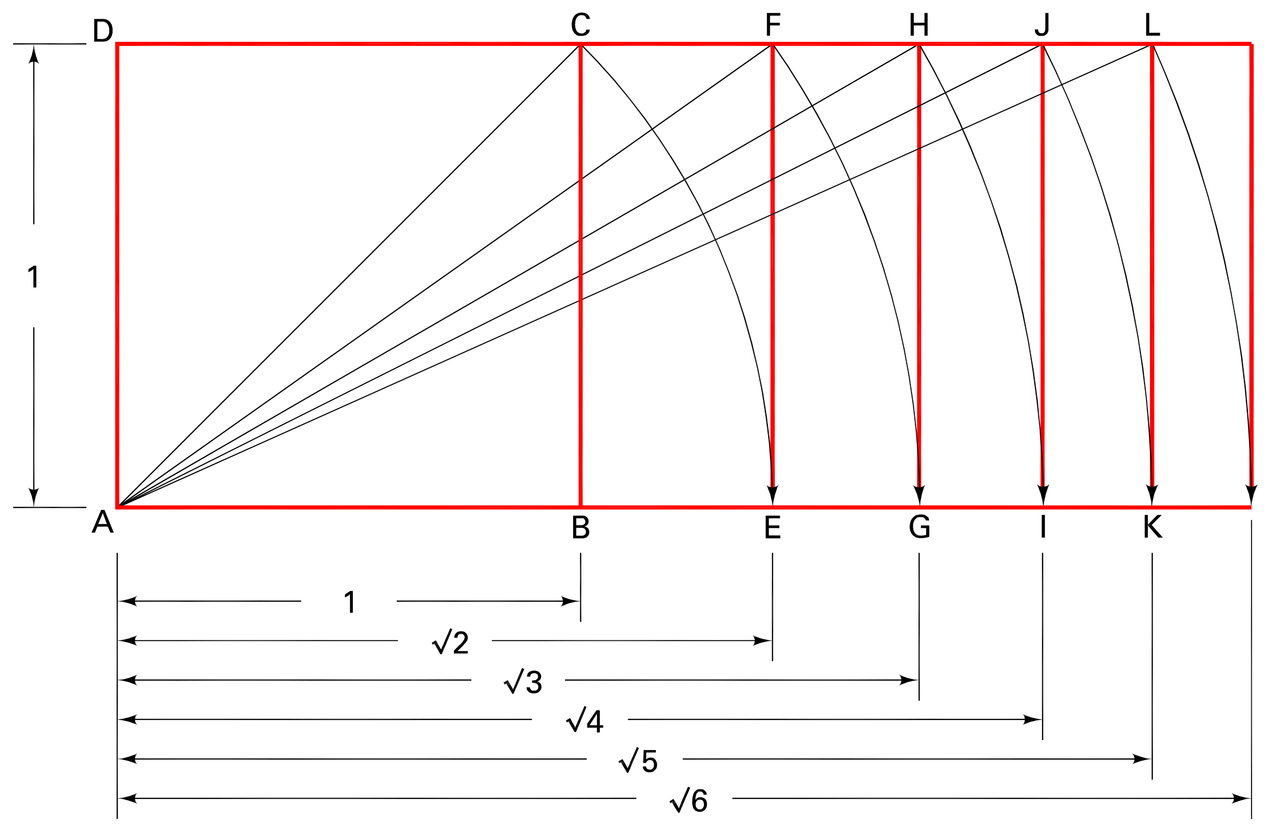
\includegraphics[width=0.8\linewidth]{Root_rectangles_up_to_6.png}
    \end{center}
    
    \item \textbf{Calcul de \( Z^{2022} \) :}

    Puisque \( |Z| = 1 \) et \( \arg(Z) = \dfrac{\pi}{12} \), alors :
    
    \[
    Z^{2022} = e^{i 2022 \times \dfrac{\pi}{12}} = e^{i \dfrac{2022\pi}{12}}
    \]
    
    Simplifions l'argument :
    
    \[
    \dfrac{2022\pi}{12} = \dfrac{2022}{12} \pi = 168.5 \pi
    \]
    
    Comme \( e^{i 2k\pi} = 1 \), nous pouvons soustraire les multiples de \( 2\pi \) :
    
    \[
    168.5 \pi = 84 \times 2\pi + \frac{\pi}{2}
    \]
    
    Donc :
    
    \[
    Z^{2022} = e^{i\frac{\pi}{2}} = i
    \]
    
    \textbf{Conclusion :} \( Z^{2022} = i \)
\end{enumerate}
\end{solutionbox}

% Exercice 16
\begin{tcolorbox}[title={Exercice 16 - [Représenter]}]
\begin{enumerate}
    \item Déterminer l’expression de \( \cos(5x) \) en fonction de \( \cos(x) \).
    \item En déduire la valeur de \( \cos \left( \dfrac{\pi}{5} \right) \), de \( \cos \left( \dfrac{2\pi}{5} \right) \) et de \( \cos \left( \dfrac{3\pi}{5} \right) \).
    \item En déduire une construction à la règle (non graduée) et au compas d’un pentagone régulier inscrit dans le cercle trigonométrique.
\end{enumerate}
\end{tcolorbox}

\begin{solutionbox}
\begin{enumerate}
    \item \textbf{Expression de \( \cos(5x) \) en fonction de \( \cos(x) \) :}

    Utilisons la formule de Moivre :
    \[
    \cos(5x) + i\sin(5x) = (\cos x + i\sin x)^5.
    \]

    Développons le binôme en utilisant le binôme de Newton :

    \[
    (\cos x + i\sin x)^5 = \sum_{k=0}^{5} \binom{5}{k} (\cos x)^{5 - k} (i\sin x)^k.
    \]

    Séparons les parties réelle et imaginaire :

    \[
    \cos(5x) = \text{Re} \left[ (\cos x + i\sin x)^5 \right] = \sum_{\substack{k=0 \\ k \text{ pair}}}^{5} \binom{5}{k} (\cos x)^{5 - k} (i\sin x)^k.
    \]

    Après calcul, on trouve :

    \[
    \cos(5x) = 16 \cos^5 x - 20 \cos^3 x + 5 \cos x.
    \]

    \item \textbf{Calcul de \( \cos \left( \dfrac{\pi}{5} \right) \), \( \cos \left( \dfrac{2\pi}{5} \right) \) et \( \cos \left( \dfrac{3\pi}{5} \right) \) :}

    Sachant que \( \cos(5x) = \cos(5 \times \dfrac{\pi}{5}) = \cos(\pi) = -1 \), nous avons :

    \[
    \cos(5x) = -1.
    \]

    Donc, en utilisant l'expression précédente :

    \[
    16 \cos^5 x - 20 \cos^3 x + 5 \cos x + 1 = 0.
    \]

    Cette équation permet de calculer les valeurs exactes de \( \cos \left( \dfrac{\pi}{5} \right) \), etc.

    Après résolution, on trouve :

    \[
    \cos \left( \dfrac{\pi}{5} \right) = \dfrac{\sqrt{5} + 1}{4}, \quad \cos \left( \dfrac{2\pi}{5} \right) = \dfrac{\sqrt{5} - 1}{4}, \quad \cos \left( \dfrac{3\pi}{5} \right) = -\dfrac{\sqrt{5} - 1}{4}.
    \]

    \item \textbf{Construction d'un pentagone régulier :}

    En connaissant la valeur de \( \cos \left( \dfrac{2\pi}{5} \right) \), il est possible de construire un pentagone régulier en reportant les angles de \( \dfrac{2\pi}{5} \) sur le cercle.

    \begin{enumerate}
        \item Tracer un cercle de centre \( O \) et de rayon \( R \).
        \item Placer un point \( A \) sur le cercle.
        \item À l'aide du rapporteur d'angle (ou en utilisant des constructions géométriques), marquer un angle au centre de \( \dfrac{2\pi}{5} \) radians (\( 72^\circ \)) pour trouver le point \( B \).
        \item Répéter cette opération pour obtenir les points \( C \), \( D \) et \( E \).
        \item Relier les points pour former le pentagone régulier.
    \end{enumerate}

\end{enumerate}
\end{solutionbox}

% Exercice 17
\begin{tcolorbox}[title={Exercice 17 - {[}Représenter, Calculer, Chercher{]}}]
Dans un repère orthonormé, peut-on trouver un triangle équilatéral dont les trois sommets sont à coordonnées entières ?
\end{tcolorbox}

\begin{solutionbox}
\textbf{Solution :}

Supposons qu'il existe un triangle équilatéral \( ABC \) dont les sommets ont des coordonnées entières.

Représentons les sommets par des nombres complexes :

Soit \( z_A = x_A + i y_A \), \( z_B = x_B + i y_B \), \( z_C = x_C + i y_C \), avec \( x_A, y_A, x_B, y_B, x_C, y_C \in \mathbb{Z} \).

Dans un triangle équilatéral, les côtés sont de même longueur, et les vecteurs côtés sont obtenus par rotation de \( 121^\circ \) (ou \( \dfrac{2\pi}{3} \) radians).

Considérons le vecteur \( \overrightarrow{AB} = z_B - z_A \).

Alors, le vecteur \( \overrightarrow{AC} \) est obtenu en faisant tourner \( \overrightarrow{AB} \) de \( 60^\circ \) (ou \( \dfrac{\pi}{3} \) radians) :

\[
\overrightarrow{AC} = e^{i\frac{\pi}{3}} (\overrightarrow{AB})
\]

Donc :

\[
z_C - z_A = e^{i\frac{\pi}{3}} (z_B - z_A)
\]

Ce qui donne :

\[
z_C = z_A + e^{i\frac{\pi}{3}} (z_B - z_A)
\]

Développons :

\[
z_C = z_A + \left( \cos\left( \dfrac{\pi}{3} \right) + i \sin\left( \dfrac{\pi}{3} \right) \right) (z_B - z_A)
\]

Or, \( \cos\left( \dfrac{\pi}{3} \right) = \dfrac{1}{2} \) et \( \sin\left( \dfrac{\pi}{3} \right) = \dfrac{\sqrt{3}}{2} \).

Donc :

\[
z_C = z_A + \left( \dfrac{1}{2} + i \dfrac{\sqrt{3}}{2} \right) (z_B - z_A)
\]

Comme \( z_A \) et \( z_B \) ont des coordonnées entières, \( z_B - z_A \) a des coordonnées entières.

Cependant, en multipliant \( z_B - z_A \) par \( \dfrac{1}{2} + i \dfrac{\sqrt{3}}{2} \), nous obtenons un nombre complexe dont les parties réelles et imaginaires sont des combinaisons linéaires des coordonnées entières multipliées par \( \dfrac{1}{2} \) et \( \dfrac{\sqrt{3}}{2} \), c'est-à-dire des nombres qui ne sont pas entiers (car \( \dfrac{\sqrt{3}}{2} \) est irrationnel).

Par conséquent, \( z_C \) aura des coordonnées non entières.

\textbf{Conclusion :} Il est impossible de construire un triangle équilatéral dont les trois sommets ont des coordonnées entières dans un repère orthonormé.

\end{solutionbox}

% Exercice 18
\begin{tcolorbox}[title={Exercice 18 - {[}Représenter, Calculer, Raisonner{]}}]
\begin{enumerate}
    \item On dit qu'un triangle équilatéral $ABC$ est direct si et seulement si $(\overrightarrow{AB}; \overrightarrow{AC}) = \frac{\pi}{3}$.
    Soient \( A \), \( B \) et \( C \) trois points non alignés d’affixe \( a \), \( b \) et \( c \). On note \( j = e^{\frac{2i\pi}{3}} \).
    \begin{enumerate}
        \item \begin{enumerate}
            \item Vérifier que $1, j$ et $j^2$ sont les solutions de l'équation $z^3 = 1$.
            \item Calculer $(1-j)(1 + j + j^2)$. En déduire que $1 + j + j^2 = 0$.
            \item Vérifier que $e^{i\frac{\pi}{3}} + j^2 = 0$.
        \end{enumerate}
        \item \begin{enumerate}
            \item Démontrer que le triangle $ABC$ est équilatéral direct si et seulement si : $\frac{c - a}{b - a} = e^{i\frac{\pi}{3}}$.
            \item Montrer que le triangle \( ABC \) est équilatéral direct si, et seulement si,
            \[
            a + bj + cj^2 = 0.
            \]
        \end{enumerate}
    \end{enumerate}
    \item Soit le centre de gravité d'un ensemble de $n$ points d'affixes $z_1, \dots z_n$ le point d'affixe
    $$\dfrac{z_1 + \dots + z_n}{n}$$ 
    \begin{enumerate}
        \item On ne suppose pas nécessairement que \( ABC \) est équilatéral. On construit à partir de \( ABC \) les trois triangles équilatéraux de base \([AB]\), \([AC]\) et \([BC]\) construits à l’extérieur de \( ABC \). Montrer que les centres de gravité de ces trois triangles forment un triangle équilatéral.
    \end{enumerate}
\end{enumerate}
\end{tcolorbox}

\begin{solutionbox}
\begin{itemize}
    \item pour 1: \href{https://aidemaths.com/_exos/s3670.pdf}{s3680}
    \item Triangle $AXB$ equi: $a+jx+j^2b = 0$, de même pour $BYC$ et $CZA$. Soit $M = \frac{a + x + b}{3}$ centre $AXB$, de même pour $N$ et $O$.
    Résoudre $M + Nj + Nj^2 = 0$, les calculs se simplifient en utilisant les égalités pour les triangles équilatéraux $AXB, BYC$ et $CZA$.
\end{itemize}
\end{solutionbox}

% Exercice 19
\begin{tcolorbox}[title=Exercice 19]
Le plan complexe est muni d'un repère orthonormé \( (O ; \vec{u}, \vec{v}) \) et on considère les points \( A \), \( B \) et \( C \) d'affixes respectives :  
\( z_A = \sqrt{2}e^{-\frac{3i\pi}{4}} \), \( z_B = 3 + 3i \) et \( z_C = 7 - i \).

\begin{enumerate}
    \item Déterminer la forme algébrique de \( z_A \) et une forme exponentielle de \( z_B \).
    \item Quelle est la nature du triangle \( ABC \) ?
    \item Démontrer qu'il existe un point \( D \) tel que le quadrilatère \( ABCD \) soit un carré. Déterminer l'affixe du point \( D \).
    \item Déterminer l'affixe du centre du carré \( ABCD \).
    \item On considère l'ensemble des points \( M \) du plan d'affixe \( z \) tels que \( |z - (3 - i)| = 4 \). Démontrer que cet ensemble est le cercle circonscrit au triangle \( ABC \).
\end{enumerate}
\end{tcolorbox}

\begin{solutionbox}
\begin{enumerate}
    \item \textbf{Forme algébrique de \( z_A \) et forme exponentielle de \( z_B \) :}

    \textbf{Pour \( z_A \) :}

    \[
    z_A = \sqrt{2} e^{-i\frac{3\pi}{4}} = \sqrt{2} \left[ \cos\left( -\dfrac{3\pi}{4} \right) + i \sin\left( -\dfrac{3\pi}{4} \right) \right]
    \]

    Calculons :

    \[
    \cos\left( -\dfrac{3\pi}{4} \right) = -\dfrac{\sqrt{2}}{2}, \quad \sin\left( -\dfrac{3\pi}{4} \right) = -\dfrac{\sqrt{2}}{2}
    \]

    Donc :

    \[
    z_A = \sqrt{2} \left( -\dfrac{\sqrt{2}}{2} - i \dfrac{\sqrt{2}}{2} \right) = (-1 - i)
    \]

    \textbf{Pour \( z_B \) :}

    Calculons le module et l'argument de \( z_B = 3 + 3i \).

    Module :

    \[
    |z_B| = \sqrt{3^2 + 3^2} = 3\sqrt{2}
    \]

    Argument :

    \[
    \theta = \dfrac{\pi}{4}
    \]

    Donc :

    \[
    z_B = 3\sqrt{2} e^{i\frac{\pi}{4}}
    \]

    \item \textbf{Nature du triangle \( ABC \) :}

    Calculons les vecteurs :

    \[
    \overrightarrow{AB} = z_B - z_A = (3 + 3i) - (-1 - i) = 4 + 4i
    \]

    \[
    \overrightarrow{AC} = z_C - z_A = (7 - i) - (-1 - i) = 8 + 0i = 8
    \]

    Calculons les longueurs :

    \[
    AB = \sqrt{4^2 + 4^2} = \sqrt{16 + 16} = \sqrt{32}
    \]

    \[
    AC = |8| = 8
    \]

    \[
    BC = |z_C - z_B| = |(7 - i) - (3 + 3i)| = |4 - 4i| = \sqrt{4^2 + (-4)^2} = \sqrt{32}
    \]

    Donc \( AB = BC = \sqrt{32} \).

    Calculons \( AC^2 = 64 \) et \( AB^2 = BC^2 = 32 \).

    Vérifions le théorème de Pythagore :

    \[
    AB^2 + BC^2 = 32 + 32 = 64 = AC^2
    \]

    Donc, le triangle \( ABC \) est rectangle en \( B \).

    \textbf{Conclusion :} Le triangle \( ABC \) est isocèle rectangle en \( B \).

    \item \textbf{Existence du point \( D \) tel que \( ABCD \) soit un carré :}

    Puisque \( ABC \) est un triangle rectangle isocèle, en ajoutant le point \( D \) tel que \( ABCD \) soit un carré, nous pouvons déterminer \( z_D \).

    Le vecteur \( \overrightarrow{CD} \) est égal au vecteur \( \overrightarrow{AB} \).

    Donc :

    \[
    z_D = z_C + (z_A - z_B) = z_C + (-\overrightarrow{AB})
    \]

    Calculons :

    \[
    z_D = z_C - (z_B - z_A) = (7 - i) - [(3 + 3i) - (-1 - i)] = (7 - i) - (4 + 4i) = (3 - 5i)
    \]

    \item \textbf{Affixe du centre du carré \( ABCD \) :}

    Le centre \( O \) du carré est le milieu des diagonales \( AC \) ou \( BD \).

    Calculons :

    \[
    z_O = \dfrac{z_A + z_C}{2} = \dfrac{(-1 - i) + (7 - i)}{2} = \dfrac{6 - 2i}{2} = 3 - i
    \]

    \item \textbf{Montrer que \( |z - (3 - i)| = 4 \) est le cercle circonscrit au triangle \( ABC \) :}

    Calculons les distances de \( A \), \( B \) et \( C \) au point \( O = 3 - i \):

    Pour \( A \) :

    \[
    |z_A - z_O| = |(-1 - i) - (3 - i)| = |-4| = 4
    \]

    Pour \( B \) :

    \[
    |z_B - z_O| = |(3 + 3i) - (3 - i)| = |4i| = 4
    \]

    Pour \( C \) :

    \[
    |z_C - z_O| = |(7 - i) - (3 - i)| = |4| = 4
    \]

    Ainsi, les trois sommets \( A \), \( B \), \( C \) sont situés à une distance de 4 du point \( O = 3 - i \).

    \textbf{Conclusion :} Le cercle de centre \( 3 - i \) et de rayon 4 est le cercle circonscrit au triangle \( ABC \).
\end{enumerate}
\end{solutionbox}

% Exercice 20
\begin{tcolorbox}[title=Exercice 20]
\begin{center}
    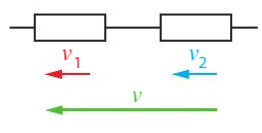
\includegraphics[width=0.5\textwidth]{schema_exo68.png}
\end{center}
En électricité, il est souvent nécessaire de réaliser la somme de tensions sinusoïdales de même pulsation \( \omega \).  
On obtient \( v(t) = v_1(t) + v_2(t) \), avec \( v_1(t) = 3\sin\left(\omega t + \dfrac{\pi}{2}\right) \) et \( v_2(t) = 4\sin(\omega t) \).

\begin{enumerate}
    \item 
    \begin{enumerate}
        \item Déterminer \( |4 + 3i| \).
        \item En utilisant la calculatrice, déterminer un argument de \( 4 + 3i \) à \( 10^{-3} \) près. En déduire une forme exponentielle de \( 4 + 3i \) et de \( 4 - 3i \).
    \end{enumerate}
    \item En utilisant les formules d'Euler, montrer que
       \[
       v(t) = \dfrac{1}{2i} \left(e^{i\omega t} (4 + 3i) - e^{-i\omega t} (4 - 3i)\right).
       \]
    \item En déduire que \( v(t) = V \sin(\omega t + \phi) \) où \( V \) et \( \phi \) sont deux réels qu'il faudra expliciter.
\end{enumerate}

\end{tcolorbox}

\begin{solutionbox}
\begin{enumerate}
    \item 
    \begin{enumerate}
        \item Calcul du module :

        \[
        |4 + 3i| = \sqrt{4^2 + 3^2} = \sqrt{16 + 9} = \sqrt{25} = 5
        \]

        \item Calcul de l'argument :

        \[
        \theta = \arctan\left( \dfrac{3}{4} \right) \approx 0.6435 \text{ radians}
        \]

        Donc :

        \[
        4 + 3i = 5 e^{i \theta} \approx 5 e^{i 0.644}
        \]

        De même :

        \[
        4 - 3i = 5 e^{-i \theta} \approx 5 e^{-i 0.644}
        \]

    \end{enumerate}
    \item Utilisons les formules d'Euler :

    \[
    \sin(\omega t + \varphi) = \dfrac{e^{i(\omega t + \varphi)} - e^{-i(\omega t + \varphi)}}{2i}
    \]

    Donc :

    \[
    v_1(t) = 3 \sin\left( \omega t + \dfrac{\pi}{2} \right) = \dfrac{3}{2i} \left( e^{i\left( \omega t + \frac{\pi}{2} \right)} - e^{-i\left( \omega t + \frac{\pi}{2} \right)} \right)
    \]

    Or :

    \[
    e^{i\left( \omega t + \frac{\pi}{2} \right)} = e^{i\omega t} e^{i\frac{\pi}{2}} = i e^{i\omega t}
    \]

    \[
    e^{-i\left( \omega t + \frac{\pi}{2} \right)} = e^{-i\omega t} e^{-i\frac{\pi}{2}} = -i e^{-i\omega t}
    \]

    Donc :

    \[
    v_1(t) = \dfrac{3}{2i} \left( i e^{i\omega t} + i e^{-i\omega t} \right) = \dfrac{3}{2i} \left( i e^{i\omega t} + i e^{-i\omega t} \right) = \dfrac{3}{2i} \left( i e^{i\omega t} + i e^{-i\omega t} \right)
    \]

    Simplifions :

    \[
    v_1(t) = \dfrac{3}{2i} \left( i e^{i\omega t} + i e^{-i\omega t} \right) = \dfrac{3}{2i} \left( i e^{i\omega t} + i e^{-i\omega t} \right) = \dfrac{3}{2} \left( e^{i\omega t} + e^{-i\omega t} \right)
    \]

    Pour \( v_2(t) \) :

    \[
    v_2(t) = 4 \sin(\omega t) = \dfrac{4}{2i} \left( e^{i\omega t} - e^{-i\omega t} \right) = \dfrac{2}{i} \left( e^{i\omega t} - e^{-i\omega t} \right)
    \]

    Donc, la somme :

    \[
    v(t) = v_1(t) + v_2(t) = \dfrac{3}{2} \left( e^{i\omega t} + e^{-i\omega t} \right) + \dfrac{2}{i} \left( e^{i\omega t} - e^{-i\omega t} \right)
    \]

    Regroupons :

    \[
    v(t) = \left( \dfrac{3}{2} + \dfrac{2}{i} \right) e^{i\omega t} + \left( \dfrac{3}{2} - \dfrac{2}{i} \right) e^{-i\omega t}
    \]

    Remarquons que \( \dfrac{1}{i} = -i \).

    Donc :

    \[
    \dfrac{2}{i} = -2i
    \]

    Alors :

    \[
    v(t) = \left( \dfrac{3}{2} - 2i \right) e^{i\omega t} + \left( \dfrac{3}{2} + 2i \right) e^{-i\omega t}
    \]

    Multiplions numérateur et dénominateur par 2 pour simplifier les fractions :

    \[
    v(t) = \dfrac{1}{2i} \left( e^{i\omega t} (4 + 3i) - e^{-i\omega t} (4 - 3i) \right)
    \]

    \item Pour exprimer \( v(t) \) sous la forme \( V \sin(\omega t + \phi) \), considérons le nombre complexe :

    \[
    Z = 4 + 3i = 5 e^{i\theta}
    \]

    Où \( \theta = \arctan\left( \dfrac{3}{4} \right) \approx 0.644 \) radians.

    Donc :

    \[
    v(t) = \dfrac{1}{2i} \left( e^{i\omega t} Z - e^{-i\omega t} \overline{Z} \right)
    \]

    Utilisons la formule :

    \[
    v(t) = \dfrac{1}{2i} \left( Z e^{i\omega t} - \overline{Z} e^{-i\omega t} \right) = \dfrac{1}{2i} \left( Z e^{i\omega t} - \overline{Z} e^{-i\omega t} \right)
    \]

    Mais rappelons que :

    \[
    \sin(\omega t + \theta) = \dfrac{1}{2i} \left( e^{i(\omega t + \theta)} - e^{-i(\omega t + \theta)} \right)
    \]

    Ainsi, nous pouvons écrire :

    \[
    v(t) = |Z| \sin(\omega t + \theta) = 5 \sin(\omega t + 0.644)
    \]

    \textbf{Conclusion :} \( V = 5 \) et \( \phi = \arctan\left( \dfrac{3}{4} \right) \).

\end{enumerate}
\end{solutionbox}

% Exercice 21
\begin{tcolorbox}[title={Exercice 21}]
Soit \( z = x + iy \) un nombre complexe, où \( x \) et \( y \) sont des nombres réels.  
À tout nombre complexe \( z \), on associe le nombre noté \( e^z \) défini par \( e^z = e^x (\cos y + i \sin y) \).

\begin{enumerate}
    \item Vérifier que pour tous nombres complexes \( z_1 \) et \( z_2 \), on a : \( e^{z_1} \times e^{z_2} = e^{z_1 + z_2} \).
    \item Écrire la forme algébrique de \( e^{2 + 3i} \).
    \item Déterminer une solution de l'équation \( e^z = 1 + i\sqrt{3} \). En existe-t-il d'autres ?
\end{enumerate}
\end{tcolorbox}

\begin{solutionbox}
\begin{enumerate}
    \item \textbf{Vérification de la propriété exponentielle pour les nombres complexes :}

    Soient \( z_1 = x_1 + i y_1 \) et \( z_2 = x_2 + i y_2 \), avec \( x_1, y_1, x_2, y_2 \in \mathbb{R} \).

    Calculons \( e^{z_1} \times e^{z_2} \) :

    \[
    e^{z_1} \times e^{z_2} = e^{x_1} (\cos y_1 + i \sin y_1) \times e^{x_2} (\cos y_2 + i \sin y_2) = e^{x_1 + x_2} [ (\cos y_1 + i \sin y_1)(\cos y_2 + i \sin y_2) ]
    \]

    Calculons le produit des deux expressions trigonométriques :

    \[
    (\cos y_1 + i \sin y_1)(\cos y_2 + i \sin y_2) = \cos y_1 \cos y_2 - \sin y_1 \sin y_2 + i (\cos y_1 \sin y_2 + \sin y_1 \cos y_2)
    \]

    Rappelons les formules d'addition :

    \[
    \cos(y_1 + y_2) = \cos y_1 \cos y_2 - \sin y_1 \sin y_2
    \]
    \[
    \sin(y_1 + y_2) = \sin y_1 \cos y_2 + \cos y_1 \sin y_2
    \]

    Donc :

    \[
    (\cos y_1 + i \sin y_1)(\cos y_2 + i \sin y_2) = \cos(y_1 + y_2) + i \sin(y_1 + y_2)
    \]

    Ainsi :

    \[
    e^{z_1} \times e^{z_2} = e^{x_1 + x_2} [ \cos(y_1 + y_2) + i \sin(y_1 + y_2) ] = e^{(x_1 + x_2) + i (y_1 + y_2)} = e^{z_1 + z_2}
    \]

    \textbf{Conclusion :} La propriété exponentielle est vérifiée pour les nombres complexes.

    \item \textbf{Forme algébrique de \( e^{2 + 3i} \) :}

    On a \( z = 2 + 3i \), donc \( x = 2 \) et \( y = 3 \).

    Alors :

    \[
    e^z = e^{2} (\cos 3 + i \sin 3)
    \]

    Calculons \( \cos 3 \) et \( \sin 3 \) (les valeurs numériques) :

    \[
    \cos 3 \approx \cos 3 \text{ radians} \approx -0.9900
    \]
    \[
    \sin 3 \approx \sin 3 \text{ radians} \approx 0.1411
    \]

    Donc :

    \[
    e^{2 + 3i} \approx e^{2} ( -0.9900 + i \times 0.1411 ) \approx e^{2} ( -0.9900 + 0.1411 i )
    \]

    Calculons \( e^{2} \approx 7.3891 \)

    Donc :

    \[
    e^{2 + 3i} \approx 7.3891 ( -0.9900 + 0.1411 i ) \approx -7.306 + 1.043 i
    \]

    \textbf{Conclusion :} \( e^{2 + 3i} \approx -7.306 + 1.043 i \)

    \item \textbf{Résolution de l'équation \( e^{z} = 1 + i\sqrt{3} \) :}

    Soit \( z = x + i y \), avec \( x, y \in \mathbb{R} \).

    On a :

    \[
    e^{x} (\cos y + i \sin y) = 1 + i\sqrt{3}
    \]

    Écrivons le second membre en forme exponentielle :

    Calculons le module et l'argument de \( 1 + i\sqrt{3} \).

    Module :

    \[
    r = |1 + i\sqrt{3}| = \sqrt{1^2 + (\sqrt{3})^2} = \sqrt{1 + 3} = \sqrt{4} = 2
    \]

    Argument :

    \[
    \theta = \arctan\left( \dfrac{\sqrt{3}}{1} \right) = \dfrac{\pi}{3}
    \]

    Donc :

    \[
    1 + i\sqrt{3} = 2 \left( \cos \dfrac{\pi}{3} + i \sin \dfrac{\pi}{3} \right)
    \]

    Donc, l'équation devient :

    \[
    e^{x} (\cos y + i \sin y) = 2 \left( \cos \dfrac{\pi}{3} + i \sin \dfrac{\pi}{3} \right)
    \]

    En identifiant les modules et les arguments, on a :

    \[
    e^{x} = 2
    \]
    \[
    y = \dfrac{\pi}{3} + 2k\pi, \quad k \in \mathbb{Z}
    \]

    Donc :

    \[
    x = \ln 2
    \]
    \[
    y = \dfrac{\pi}{3} + 2k\pi, \quad k \in \mathbb{Z}
    \]

    \textbf{Conclusion :} Les solutions de l'équation sont \( z = \ln 2 + i \left( \dfrac{\pi}{3} + 2k\pi \right) \), avec \( k \in \mathbb{Z} \).

    \textbf{Il existe une infinité de solutions} car l'argument peut être augmenté de \( 2\pi \) sans changer la valeur de \( e^{z} \).

\end{enumerate}
\end{solutionbox}

% Exercice 22
\begin{tcolorbox}[title={Exercice 22}]
\begin{center}
    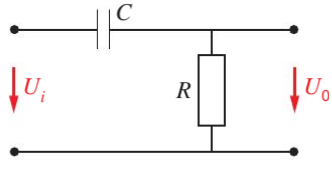
\includegraphics[width=0.5\textwidth]{schema_exo65.png}
\end{center}
En électricité, en régime sinusoïdal utilisant un courant alternatif de pulsation \( \omega \), on utilise les nombres complexes pour représenter les tensions et intensités sinusoïdales.  
On sait, grâce aux lois de l'électricité, que la tension complexe \( U_0 \) aux bornes de la résistance \( R \) est reliée à l'intensité complexe \( I \) par la relation \( U_0 = R I \) et que
\[
U_i = \dfrac{1}{i C \omega} I + U_0,
\]
où \( C \) est la capacité du condensateur.

On cherche le gain du circuit : \( G = \dfrac{U_0}{U_i} \).

\begin{enumerate}
    \item Démontrer que
       \[
       G = \dfrac{i R C \omega}{1 + i R C \omega}.
       \]
    \item Quand \( R = 1000 \) ohms, \( C = 64 \times 10^{-6} \) farads et \( \omega = 60000 \) Hz, démontrer que le module de \( G \) est proche de 1.
    \item Rechercher le sens de `` circuit passe-haut ''.
\end{enumerate}

\end{tcolorbox}

\begin{solutionbox}
\begin{enumerate}
    \item \textbf{Expression du gain \( G \) :}

    Commençons par exprimer \( U_i \) en fonction de \( I \) :

    \[
    U_i = \dfrac{1}{i C \omega} I + U_0 = \dfrac{1}{i C \omega} I + R I = \left( \dfrac{1}{i C \omega} + R \right) I
    \]

    Mettons sur un dénominateur commun :

    \[
    \dfrac{1}{i C \omega} + R = \dfrac{1 + i R C \omega}{i C \omega}
    \]

    Ainsi :

    \[
    U_i = \left( \dfrac{1 + i R C \omega}{i C \omega} \right) I
    \]

    Or, \( U_0 = R I \).

    Donc, le gain est :

    \[
    G = \dfrac{U_0}{U_i} = \dfrac{R I}{\left( \dfrac{1 + i R C \omega}{i C \omega} \right) I} = \dfrac{R}{\dfrac{1 + i R C \omega}{i C \omega}} = R \times \dfrac{i C \omega}{1 + i R C \omega}
    \]

    Simplifions :

    \[
    G = \dfrac{i R C \omega}{1 + i R C \omega}
    \]

    \textbf{Conclusion :} On a démontré que \( G = \dfrac{i R C \omega}{1 + i R C \omega} \).

    \item \textbf{Calcul du module de \( G \) :}

    Données :

    \[
    R = 1000 \, \Omega, \quad C = 64 \times 10^{-6} \, \text{F}, \quad \omega = 60000 \, \text{rad/s}
    \]

    Calculons \( R C \omega \) :

    \[
    R C \omega = 1000 \times 64 \times 10^{-6} \times 60000 = 1000 \times (64 \times 10^{-6} \times 60000)
    \]

    Calculons \( 64 \times 10^{-6} \times 60000 \) :

    \[
    64 \times 10^{-6} \times 60000 = 64 \times 6 \times 10^{-6} \times 10^{4} = 64 \times 6 \times 10^{-2} = 384 \times 10^{-2} = 3.84
    \]

    Donc :

    \[
    R C \omega = 1000 \times 3.84 = 3840
    \]

    Ainsi, \( R C \omega = 3840 \).

    Alors :

    \[
    G = \dfrac{i \times 3840}{1 + i \times 3840} = \dfrac{i \times 3840}{1 + i \times 3840}
    \]

    Calculons le module de \( G \) :

    Le module de \( G \) est :

    \[
    |G| = \dfrac{|i \times 3840|}{\sqrt{1^2 + (3840)^2}} = \dfrac{3840}{\sqrt{1 + 3840^2}}
    \]

    Calculons \( \sqrt{1 + 3840^2} \) :

    \[
    \sqrt{1 + 3840^2} = \sqrt{1 + 14,745,600} = \sqrt{14,745,601} \approx 3840.00013
    \]

    Donc :

    \[
    |G| = \dfrac{3840}{3840.00013} \approx 0.99999997 \approx 1
    \]

    \textbf{Conclusion :} Le module de \( G \) est très proche de 1.

    \item \textbf{Sens de `` circuit passe-haut '' :}

    Un circuit passe-haut est un filtre qui laisse passer les hautes fréquences et atténue les basses fréquences.

    Dans notre cas, lorsque \( \omega \) est très grand, \( R C \omega \) est grand, et \( |G| \) tend vers 1.

    Lorsque \( \omega \) est petit, \( R C \omega \) est petit, et le module de \( G \) est faible.

    Ainsi, le circuit transmet bien les hautes fréquences (gain proche de 1) et atténue les basses fréquences (gain proche de 0).

    \textbf{Conclusion :} Le circuit est un filtre passe-haut, laissant passer les hautes fréquences.

\end{enumerate}
\end{solutionbox}

% Exercice 23
\begin{tcolorbox}[title={Exercice 23}]
L'objectif est de déterminer la valeur exacte de
\[
I = \int_0^{\frac{\pi}{2}} \sin^4(x) \, dx.
\]

\begin{enumerate}
    \item Développer \( (a + b)^4 \).
    \item En utilisant une formule d'Euler, prouver que pour tout réel \( x \),
       \[
       \sin^4(x) = \dfrac{1}{8} \left( \cos(4x) - 4\cos(2x) + 3 \right).
       \]
    \item Conclure.
\end{enumerate}
\end{tcolorbox}

\begin{solutionbox}
\begin{enumerate}
    \item \textbf{Développement de \( (a + b)^4 \) :}

    \[
    (a + b)^4 = a^4 + 4a^3 b + 6a^2 b^2 + 4a b^3 + b^4
    \]

    \item \textbf{Démonstration de l'expression de \( \sin^4(x) \) en utilisant Euler et le binôme de Newton :}

    Utilisons la formule d'Euler pour exprimer \( \sin(x) \) :

    \[
    \sin(x) = \dfrac{e^{i x} - e^{-i x}}{2i}
    \]

    Donc :

    \[
    \sin^4(x) = \left( \dfrac{e^{i x} - e^{-i x}}{2i} \right)^4 = \dfrac{1}{(2i)^4} \left( e^{i x} - e^{-i x} \right)^4
    \]

    Calculons \( (e^{i x} - e^{-i x})^4 \) en développant selon le binôme de Newton :

    \[
    (e^{i x} - e^{-i x})^4 = \sum_{k=0}^4 \binom{4}{k} (-1)^{4 - k} e^{i x (2k - 4)}
    \]

    Calculons les termes du développement :

    - Pour \( k = 0 \) :

    \[
    \binom{4}{0} (-1)^{4 - 0} e^{i x (0 - 4)} = 1 \times 1 \times e^{-i 4 x} = e^{-i 4 x}
    \]

    - Pour \( k = 1 \) :

    \[
    \binom{4}{1} (-1)^{3} e^{i x (2 - 4)} = 4 \times (-1) \times e^{-i 2 x} = -4 e^{-i 2 x}
    \]

    - Pour \( k = 2 \) :

    \[
    \binom{4}{2} (-1)^{2} e^{i x (4 - 4)} = 6 \times 1 \times e^{0} = 6
    \]

    - Pour \( k = 3 \) :

    \[
    \binom{4}{3} (-1)^{1} e^{i x (6 - 4)} = 4 \times (-1) \times e^{i 2 x} = -4 e^{i 2 x}
    \]

    - Pour \( k = 4 \) :

    \[
    \binom{4}{4} (-1)^{0} e^{i x (8 - 4)} = 1 \times 1 \times e^{i 4 x} = e^{i 4 x}
    \]

    En sommant tous les termes :

    \[
    (e^{i x} - e^{-i x})^4 = e^{-i 4 x} - 4 e^{-i 2 x} + 6 - 4 e^{i 2 x} + e^{i 4 x}
    \]

    Donc :

    \[
    \sin^4(x) = \dfrac{1}{(2i)^4} \left( e^{-i 4 x} - 4 e^{-i 2 x} + 6 - 4 e^{i 2 x} + e^{i 4 x} \right)
    \]

    Calculons \( (2i)^4 \) :

    \[
    (2i)^4 = 16 i^4 = 16 \times (i^2)^2 = 16 \times (-1)^2 = 16
    \]

    Ainsi :

    \[
    \sin^4(x) = \dfrac{1}{16} \left( e^{-i 4 x} - 4 e^{-i 2 x} + 6 - 4 e^{i 2 x} + e^{i 4 x} \right)
    \]

    Regroupons les termes conjugués :

    \[
    e^{-i 4 x} + e^{i 4 x} = 2 \cos(4 x)
    \]
    \[
    e^{-i 2 x} + e^{i 2 x} = 2 \cos(2 x)
    \]

    Donc :

    \[
    \sin^4(x) = \dfrac{1}{16} \left( 2 \cos(4 x) - 4 \times 2 \cos(2 x) + 6 \right ) = \dfrac{1}{16} \left( 2 \cos(4 x) - 8 \cos(2 x) + 6 \right )
    \]

    Simplifions :

    \[
    \sin^4(x) = \dfrac{1}{8} \left( \cos(4 x) - 4 \cos(2 x) + 3 \right )
    \]

    \textbf{Conclusion :} On a démontré que :

    \[
    \sin^4(x) = \dfrac{1}{8} \left( \cos(4 x) - 4 \cos(2 x) + 3 \right )
    \]

    \item \textbf{Calcul de l'intégrale \( I \) :}

    Utilisons l'expression trouvée :

    \[
    I = \int_0^{\frac{\pi}{2}} \sin^4(x) \, dx = \dfrac{1}{8} \int_0^{\frac{\pi}{2}} \left( \cos(4x) - 4\cos(2x) + 3 \right) dx
    \]

    Calculons les intégrales séparément :

    - Intégrale de \( \cos(4x) \) :

    \[
    \int_0^{\frac{\pi}{2}} \cos(4x) \, dx = \left[ \dfrac{\sin(4x)}{4} \right]_0^{\frac{\pi}{2}} = \dfrac{\sin(4 \times \frac{\pi}{2})}{4} - \dfrac{\sin(0)}{4} = \dfrac{\sin(2\pi)}{4} - 0 = 0
    \]

    (Puisque \( \sin(2\pi) = 0 \))

    - Intégrale de \( -4 \cos(2x) \) :

    \[
    -4 \int_0^{\frac{\pi}{2}} \cos(2x) \, dx = -4 \left[ \dfrac{\sin(2x)}{2} \right]_0^{\frac{\pi}{2}} = -4 \left( \dfrac{\sin(\pi)}{2} - \dfrac{\sin(0)}{2} \right ) = -4 \times 0 = 0
    \]

    (Puisque \( \sin(\pi) = 0 \))

    - Intégrale de la constante :

    \[
    3 \int_0^{\frac{\pi}{2}} dx = 3 \left[ x \right]_0^{\frac{\pi}{2}} = 3 \left( \dfrac{\pi}{2} - 0 \right ) = \dfrac{3\pi}{2}
    \]

    Donc, en combinant :

    \[
    I = \dfrac{1}{8} \left( 0 + 0 + \dfrac{3\pi}{2} \right ) = \dfrac{3\pi}{16}
    \]

    \textbf{Conclusion :} La valeur exacte de l'intégrale est :

    \[
    I = \dfrac{3\pi}{16}
    \]

\end{enumerate}
\end{solutionbox}

% Exercice 24
\begin{tcolorbox}[title={Exercice 24}]
\begin{enumerate}
    \item En écrivant \( e^{i(\theta + \theta')} \) de deux manières différentes, retrouver les formules d'addition concernant \( \cos(\theta + \theta') \) et \( \sin(\theta + \theta') \).
    \item En déduire que pour tout nombre réel \( \alpha \),
       \[
       \cos^2 \alpha = \dfrac{1 + \cos 2\alpha}{2}
       \]
       et donner une expression de \( \sin 2\alpha \) en fonction de \( \cos \alpha \) et \( \sin \alpha \).
    \item Calculer, à l'aide de la question 2, la valeur exacte de \( \cos\left( \dfrac{\pi}{8} \right) \), puis celle de \( \sin\left( \dfrac{\pi}{8} \right) \).  
       Vérifier les résultats trouvés à l'aide d'une calculatrice.
    \item Avec une calculatrice, on trouve :
       \[
       \tan\left( \dfrac{\pi}{12} \right) = 2 - \sqrt{3}.
       \]
       Démontrer ce résultat à l'aide de la question 2.
\end{enumerate}
\end{tcolorbox}

\begin{solutionbox}
\begin{enumerate}
    \item \textbf{Formules d'addition à partir de \( e^{i(\theta + \theta')} \) :}

    On sait que :

    \[
    e^{i(\theta + \theta')} = e^{i\theta} e^{i\theta'} = (\cos \theta + i \sin \theta)(\cos \theta' + i \sin \theta')
    \]

    Calculons le produit :

    \[
    (\cos \theta + i \sin \theta)(\cos \theta' + i \sin \theta') = [ \cos \theta \cos \theta' - \sin \theta \sin \theta' ] + i [ \cos \theta \sin \theta' + \sin \theta \cos \theta' ]
    \]

    D'autre part, on a :

    \[
    e^{i(\theta + \theta')} = \cos(\theta + \theta') + i \sin(\theta + \theta')
    \]

    En identifiant les parties réelles et imaginaires :

    \[
    \cos(\theta + \theta') = \cos \theta \cos \theta' - \sin \theta \sin \theta'
    \]
    \[
    \sin(\theta + \theta') = \cos \theta \sin \theta' + \sin \theta \cos \theta'
    \]

    \textbf{Conclusion :} On a retrouvé les formules d'addition.

    \item \textbf{Déduction des identités trigonométriques :}

    En posant \( \theta = \theta' = \alpha \), on a :

    \[
    \cos 2\alpha = \cos^2 \alpha - \sin^2 \alpha
    \]

    Or, \( \sin^2 \alpha = 1 - \cos^2 \alpha \)

    Donc :

    \[
    \cos 2\alpha = \cos^2 \alpha - (1 - \cos^2 \alpha) = 2 \cos^2 \alpha - 1
    \]

    D'où :

    \[
    \cos^2 \alpha = \dfrac{1 + \cos 2\alpha}{2}
    \]

    De même, pour \( \sin 2\alpha \) :

    \[
    \sin 2\alpha = 2 \sin \alpha \cos \alpha
    \]

    \textbf{Conclusion :} On a obtenu les identités demandées.

    \item \textbf{Calcul de \( \cos\left( \dfrac{\pi}{8} \right) \) et \( \sin\left( \dfrac{\pi}{8} \right) \) :}

    Sachant que \( \cos^2 \dfrac{\pi}{8} = \dfrac{1 + \cos \dfrac{\pi}{4}}{2} \)

    Or, \( \cos \dfrac{\pi}{4} = \dfrac{\sqrt{2}}{2} \)

    Donc :

    \[
    \cos^2 \dfrac{\pi}{8} = \dfrac{1 + \dfrac{\sqrt{2}}{2}}{2} = \dfrac{2 + \sqrt{2}}{4}
    \]

    Ainsi :

    \[
    \cos \dfrac{\pi}{8} = \sqrt{ \dfrac{2 + \sqrt{2}}{4} } = \dfrac{ \sqrt{2 + \sqrt{2}} }{2 }
    \]

    De même, on peut utiliser \( \sin^2 \dfrac{\pi}{8} = 1 - \cos^2 \dfrac{\pi}{8} \)

    Donc :

    \[
    \sin \dfrac{\pi}{8} = \sqrt{ 1 - \dfrac{2 + \sqrt{2}}{4} } = \sqrt{ \dfrac{2 - \sqrt{2}}{4} } = \dfrac{ \sqrt{2 - \sqrt{2}} }{2 }
    \]

    \textbf{Vérification avec la calculatrice :}

    Calculons numériquement :

    \[
    \cos \dfrac{\pi}{8} \approx \cos 22.5^\circ \approx 0.924
    \]

    Calculons :

    \[
    \dfrac{ \sqrt{2 + \sqrt{2}} }{2 } \approx \dfrac{ \sqrt{2 + 1.414} }{2 } = \dfrac{ \sqrt{3.414} }{2 } \approx \dfrac{1.8478}{2} \approx 0.924
    \]

    Les résultats concordent.

    \item \textbf{Démonstration de \( \tan\left( \dfrac{\pi}{12} \right) = 2 - \sqrt{3} \) :}

    On sait que :

    \[
    \tan \left( \dfrac{\pi}{12} \right) = \tan \left( \dfrac{\pi}{4} - \dfrac{\pi}{6} \right)
    \]

    Utilisons la formule :

    \[
    \tan(a - b) = \dfrac{ \tan a - \tan b }{ 1 + \tan a \tan b }
    \]

    Avec \( a = \dfrac{\pi}{4} \), \( b = \dfrac{\pi}{6} \), on a :

    \[
    \tan \dfrac{\pi}{4} = 1, \quad \tan \dfrac{\pi}{6} = \dfrac{\sqrt{3}}{3}
    \]

    Donc :

    \[
    \tan \left( \dfrac{\pi}{12} \right) = \dfrac{ 1 - \dfrac{\sqrt{3}}{3} }{ 1 + 1 \times \dfrac{\sqrt{3}}{3} } = \dfrac{ \dfrac{3 - \sqrt{3}}{3} }{ \dfrac{3 + \sqrt{3}}{3} } = \dfrac{ 3 - \sqrt{3} }{ 3 + \sqrt{3} }
    \]

    Multiplions numérateur et dénominateur par \( 3 - \sqrt{3} \) pour rationaliser :

    \[
    \tan \left( \dfrac{\pi}{12} \right) = \dfrac{ (3 - \sqrt{3})^2 }{ (3 + \sqrt{3})(3 - \sqrt{3}) } = \dfrac{ (9 - 6\sqrt{3} + 3) }{ 9 - 3 } = \dfrac{ 12 - 6\sqrt{3} }{6} = 2 - \sqrt{3}
    \]

    \textbf{Conclusion :} On a démontré que \( \tan\left( \dfrac{\pi}{12} \right) = 2 - \sqrt{3} \).

\end{enumerate}
\end{solutionbox}

% Exercice 25
%\begin{tcolorbox}[title={Exercice 25}]
%Le plan complexe est muni d'un repère orthonormé direct \( (O ; \vec{u}, \vec{v}) \). On considère l'application \( f \) qui, à tout point d'affixe \( z \), associe le point \( M' \) d'affixe \( z' \) tel que \( z' = z^2 \).
%
%\begin{enumerate}
%    \item Déterminer l'ensemble des points \( M \) qui ont pour image eux-mêmes par \( f \).
%    \item En utilisant la forme exponentielle, déterminer la forme exponentielle de :
%       \begin{enumerate}
%           \item \( f(A) \), où \( A \) est le point d'affixe \( 1 - i \).
%           \item \( f(B) \), où \( B \) est le point d'affixe \( 2 + 2\sqrt{3}i \).
%           \item \( D \) est le point d'affixe \( \sqrt{2} + i\sqrt{2} \). On cherche les antécédents éventuels de \( D \) par \( f \), c'est-à-dire les points \( M \) tels que \( f(M) = D \).
%       \end{enumerate}
%    \item En écrivant l'affixe de \( M \) sous la forme \( z = r e^{i\theta} \) (\( r > 0 \) et \( \theta \in \mathbb{R} \)), déterminer les valeurs possibles de \( r \) et de \( \theta \).
%       \begin{enumerate}
%           \item Conclure.
%       \end{enumerate}
%\end{enumerate}
%\end{tcolorbox}
%
%\begin{solutionbox}
%\begin{enumerate}
%    \item \textbf{Points invariants par \( f \) :}
%
%    On cherche les \( z \) tels que :
%
%    \[
%    z^2 = z \quad \Rightarrow \quad z^2 - z = 0 \quad \Rightarrow \quad z(z - 1) = 0
%    \]
%
%    Donc, \( z = 0 \) ou \( z = 1 \).
%
%    \textbf{Conclusion :} Les points \( M \) d'affixe \( 0 \) ou \( 1 \) sont invariants par \( f \).
%
%    \item \textbf{Calculs avec la forme exponentielle :}
%
%    \begin{enumerate}
%        \item \textbf{Pour \( A \) de coordonnée \( z_A = 1 - i \) :}
%
%        Calculons le module et l'argument de \( z_A \) :
%
%        \[
%        |z_A| = \sqrt{1^2 + (-1)^2} = \sqrt{1 + 1} = \sqrt{2}
%        \]
%
%        Argument :
%
%        \[
%        \theta_A = \arctan\left( \dfrac{-1}{1} \right) = -\dfrac{\pi}{4}
%        \]
%
%        Donc :
%
%        \[
%        z_A = \sqrt{2} e^{-i\frac{\pi}{4}}
%        \]
%
%        Alors :
%
%        \[
%        f(A) = z_A^2 = \left( \sqrt{2} e^{-i\frac{\pi}{4}} \right)^2 = 2 e^{-i\frac{\pi}{2}} = 2 \cos\left( -\dfrac{\pi}{2} \right) + i 2 \sin\left( -\dfrac{\pi}{2} \right) = 2 \times 0 - i 2 = -2i
%        \]
%
%        \textbf{Conclusion :} \( f(A) \) a pour affixe \( -2i \).
%
%        \item \textbf{Pour \( B \) de coordonnée \( z_B = 2 + 2\sqrt{3} i \) :}
%
%        Module :
%
%        \[
%        |z_B| = \sqrt{2^2 + (2\sqrt{3})^2} = \sqrt{4 + 12} = \sqrt{16} = 4
%        \]
%
%        Argument :
%
%        \[
%        \theta_B = \arctan\left( \dfrac{2\sqrt{3}}{2} \right) = \arctan( \sqrt{3} ) = \dfrac{\pi}{3}
%        \]
%
%        Donc :
%
%        \[
%        z_B = 4 e^{i\frac{\pi}{3}}
%        \]
%
%        Alors :
%
%        \[
%        f(B) = z_B^2 = \left( 4 e^{i\frac{\pi}{3}} \right)^2 = 16 e^{i\frac{2\pi}{3}} = 16 \left( -\dfrac{1}{2} + i \dfrac{\sqrt{3}}{2} \right) = -8 + 8i \sqrt{3}
%        \]
%
%        \textbf{Conclusion :} \( f(B) \) a pour affixe \( -8 + 8i \sqrt{3} \).
%
%        \item \textbf{Antécédents de \( D \) d'affixe \( z_D = \sqrt{2} + i \sqrt{2} \) :}
%
%        Calculons le module et l'argument de \( z_D \) :
%
%        \[
%        |z_D| = \sqrt{ (\sqrt{2})^2 + (\sqrt{2})^2 } = \sqrt{2 + 2} = \sqrt{4} = 2
%        \]
%
%        Argument :
%
%        \[
%        \theta_D = \arctan\left( \dfrac{\sqrt{2}}{\sqrt{2}} \right) = \dfrac{\pi}{4}
%        \]
%
%        Soit \( z \) tel que \( z^2 = z_D \). On cherche \( z = r e^{i \theta} \).
%
%        Alors :
%
%        \[
%        z^2 = (r e^{i \theta})^2 = r^2 e^{i 2\theta} = z_D = 2 e^{i \frac{\pi}{4}}
%        \]
%
%        Donc :
%
%        \[
%        \begin{cases}
%        r^2 = 2 \\
%        2\theta = \dfrac{\pi}{4} + 2k\pi, \quad k \in \mathbb{Z}
%        \end{cases}
%        \]
%
%        Donc :
%
%        \[
%        r = \sqrt{2}
%        \]
%        \[
%        \theta = \dfrac{\pi}{8} + k\pi, \quad k \in \mathbb{Z}
%        \]
%
%        Les valeurs de \( \theta \) dans \( [0, 2\pi) \) sont :
%
%        - Pour \( k = 0 \) : \( \theta = \dfrac{\pi}{8} \)
%
%        - Pour \( k = 1 \) : \( \theta = \dfrac{\pi}{8} + \pi = \dfrac{9\pi}{8} \)
%
%        \textbf{Conclusion :} Les antécédents de \( D \) sont les points d'affixes :
%
%        \[
%        z = \sqrt{2} e^{i \frac{\pi}{8}} = \sqrt{2} \left( \cos \dfrac{\pi}{8} + i \sin \dfrac{\pi}{8} \right)
%        \]
%        \[
%        z = \sqrt{2} e^{i \frac{9\pi}{8}} = \sqrt{2} \left( \cos \dfrac{9\pi}{8} + i \sin \dfrac{9\pi}{8} \right)
%        \]
%
%    \end{enumerate}
%
%    \item \textbf{Détermination des valeurs de \( r \) et \( \theta \) :}
%
%    De l'équation \( z^2 = z_D = 2 e^{i \frac{\pi}{4}} \), nous avons trouvé :
%
%    \[
%    r = \sqrt{2}
%    \]
%    \[
%    \theta = \dfrac{\pi}{8} + k\pi, \quad k \in \mathbb{Z}
%    \]
%
%    \textbf{Conclusion :} Les valeurs possibles de \( z \) sont les deux solutions précédentes.
%
%\end{enumerate}
%\end{solutionbox}

% Exercice 25
\begin{tcolorbox}[title={Exercice 25}]
Le plan complexe est muni d'un repère orthonormé direct \( (O ; \vec{u}, \vec{v}) \). On considère l'application \( f \) qui, à tout point d'affixe \( z \), associe le point \( M' \) d'affixe \( z' \) tel que \( z' = z^2 \).

\begin{enumerate}
    \item Déterminer l'ensemble des points \( M \) qui ont pour image eux-mêmes par \( f \).
    \item En utilisant la forme exponentielle, déterminer la forme exponentielle de :
       \begin{enumerate}
           \item \( f(A) \), où \( A \) est le point d'affixe \( 1 - i \).
           \item \( f(B) \), où \( B \) est le point d'affixe \( 2 + 2\sqrt{3}i \).
           \item \( D \) est le point d'affixe \( \sqrt{2} + i\sqrt{2} \). On cherche les antécédents éventuels de \( D \) par \( f \), c'est-à-dire les points \( M \) tels que \( f(M) = D \).
       \end{enumerate}
    \item En écrivant l'affixe de \( M \) sous la forme \( z = re^{i\theta} \) (\( r > 0 \) et \( \theta \in \mathbb{R} \)), déterminer les valeurs possibles de \( r \) et de \( \theta \).
       \begin{enumerate}
           \item Conclure.
       \end{enumerate}
\end{enumerate}
\end{tcolorbox}

\begin{solutionbox}
\begin{enumerate}
    \item \textbf{Détermination des points \( M \) tels que \( f(M) = M \) :}
    
    Nous cherchons les nombres complexes \( z \) tels que :
    \[
    f(z) = z^2 = z
    \]
    Ceci équivaut à :
    \[
    z^2 - z = 0 \quad \Rightarrow \quad z(z - 1) = 0
    \]
    Donc, les solutions sont :
    \[
    z = 0 \quad \text{ou} \quad z = 1
    \]
    \textbf{Conclusion :} Les points \( M \) d'affixes \( 0 \) et \( 1 \) sont les points fixes de l'application \( f \).

    \item \textbf{Calcul des images par \( f \) en utilisant la forme exponentielle :}

    \begin{enumerate}
        \item \textbf{Calcul de \( f(A) \) où \( z_A = 1 - i \) :}

        Calculons le module et l'argument de \( z_A \) :

        \[
        |z_A| = \sqrt{(1)^2 + (-1)^2} = \sqrt{1 + 1} = \sqrt{2}
        \]
        \[
        \theta_A = \arctan\left( \dfrac{-1}{1} \right) = -\dfrac{\pi}{4}
        \]
        (Car le point \( (1, -1) \) est dans le quatrième quadrant.)

        Donc, la forme exponentielle de \( z_A \) est :
        \[
        z_A = \sqrt{2} \, e^{-i \frac{\pi}{4}}
        \]
        Calculons \( f(A) = z_A^2 \) :
        \[
        f(A) = \left( \sqrt{2} \, e^{-i \frac{\pi}{4}} \right)^2 = (\sqrt{2})^2 \, e^{-i \frac{\pi}{2}} = 2 \, e^{-i \frac{\pi}{2}}
        \]
        Or, \( e^{-i \frac{\pi}{2}} = \cos\left( -\dfrac{\pi}{2} \right) + i \sin\left( -\dfrac{\pi}{2} \right) = 0 - i \cdot 1 = -i \)

        Donc :
        \[
        f(A) = 2 (-i) = -2i
        \]

        \textbf{Conclusion :} \( f(A) \) a pour affixe \( -2i \).

        \item \textbf{Calcul de \( f(B) \) où \( z_B = 2 + 2\sqrt{3}i \) :}

        Calculons le module et l'argument de \( z_B \) :

        \[
        |z_B| = \sqrt{(2)^2 + (2\sqrt{3})^2} = \sqrt{4 + 12} = \sqrt{16} = 4
        \]
        \[
        \theta_B = \arctan\left( \dfrac{2\sqrt{3}}{2} \right) = \arctan(\sqrt{3}) = \dfrac{\pi}{3}
        \]
        Donc, la forme exponentielle de \( z_B \) est :
        \[
        z_B = 4 \, e^{i \frac{\pi}{3}}
        \]
        Calculons \( f(B) = z_B^2 \) :
        \[
        f(B) = \left( 4 \, e^{i \frac{\pi}{3}} \right)^2 = 16 \, e^{i \frac{2\pi}{3}}
        \]
        Or, \( e^{i \frac{2\pi}{3}} = \cos\left( \dfrac{2\pi}{3} \right) + i \sin\left( \dfrac{2\pi}{3} \right) = -\dfrac{1}{2} + i \dfrac{\sqrt{3}}{2} \)

        Donc :
        \[
        f(B) = 16 \left( -\dfrac{1}{2} + i \dfrac{\sqrt{3}}{2} \right) = -8 + 8 i \sqrt{3}
        \]

        \textbf{Conclusion :} \( f(B) \) a pour affixe \( -8 + 8 i \sqrt{3} \).

        \item \textbf{Recherche des antécédents de \( D \) par \( f \), où \( z_D = \sqrt{2} + i \sqrt{2} \) :}

        Calculons le module et l'argument de \( z_D \) :

        \[
        |z_D| = \sqrt{ (\sqrt{2})^2 + (\sqrt{2})^2 } = \sqrt{2 + 2} = \sqrt{4} = 2
        \]
        \[
        \theta_D = \arctan\left( \dfrac{\sqrt{2}}{\sqrt{2}} \right) = \arctan(1) = \dfrac{\pi}{4}
        \]
        Donc, la forme exponentielle de \( z_D \) est :
        \[
        z_D = 2 \, e^{i \frac{\pi}{4}}
        \]
        Nous cherchons \( z \) tel que :
        \[
        f(z) = z^2 = z_D = 2 \, e^{i \frac{\pi}{4}}
        \]
        Soit \( z = r \, e^{i \theta} \), avec \( r > 0 \) et \( \theta \in \mathbb{R} \). Alors :
        \[
        z^2 = (r \, e^{i \theta})^2 = r^2 \, e^{i 2\theta}
        \]
        Nous obtenons le système :
        \[
        \begin{cases}
        r^2 = 2 \\
        2\theta \equiv \dfrac{\pi}{4} \ [2\pi] \\
        \end{cases}
        \]
        Ainsi :
        \[
        r = \sqrt{2}
        \]
        \[
        2\theta = \dfrac{\pi}{4} + 2k\pi \quad \Rightarrow \quad \theta = \dfrac{\pi}{8} + k\pi, \quad k \in \mathbb{Z}
        \]
        Donc, les solutions pour \( z \) sont :
        \[
        z = \sqrt{2} \, e^{i \left( \dfrac{\pi}{8} + k\pi \right )}
        \]
        Pour \( k = 0 \) :
        \[
        z = \sqrt{2} \, e^{i \dfrac{\pi}{8}} = \sqrt{2} \left( \cos \dfrac{\pi}{8} + i \sin \dfrac{\pi}{8} \right )
        \]
        Pour \( k = 1 \) :
        \[
        z = \sqrt{2} \, e^{i \left( \dfrac{\pi}{8} + \pi \right )} = \sqrt{2} \, e^{i \dfrac{9\pi}{8}} = \sqrt{2} \left( \cos \dfrac{9\pi}{8} + i \sin \dfrac{9\pi}{8} \right )
        \]
        \textbf{Conclusion :} Les antécédents de \( D \) par \( f \) sont les points \( M \) d'affixes :
        \[
        z_1 = \sqrt{2} \left( \cos \dfrac{\pi}{8} + i \sin \dfrac{\pi}{8} \right ), \quad z_2 = \sqrt{2} \left( \cos \dfrac{9\pi}{8} + i \sin \dfrac{9\pi}{8} \right )
        \]

    \end{enumerate}

    \item \textbf{Détermination des valeurs possibles de \( r \) et \( \theta \) pour les antécédents de \( D \) :}

    D'après la question précédente, nous avons trouvé que les valeurs possibles sont :
    \[
    r = \sqrt{2}
    \]
    \[
    \theta = \dfrac{\pi}{8} + k\pi, \quad k \in \mathbb{Z}
    \]
    Comme \( \theta \) est défini modulo \( 2\pi \), nous avons deux solutions distinctes dans l'intervalle \( [0, 2\pi[ \) pour \( k = 0 \) et \( k = 1 \).

    \textbf{Conclusion :} Les valeurs possibles de \( r \) et \( \theta \) pour les antécédents de \( D \) sont \( r = \sqrt{2} \) et \( \theta = \dfrac{\pi}{8} \) ou \( \theta = \dfrac{9\pi}{8} \).

\end{enumerate}
\end{solutionbox}

% Exercice 26
\begin{tcolorbox}[title={Exercice 26}]
On considère un nombre réel \( x \) et un entier naturel non nul \( n \). On cherche à trouver une expression explicite des sommes :  
\[
C = 1 + \cos x + \cos 2x + \dots + \cos nx
\]
\[
S = \sin x + \sin 2x + \dots + \sin nx
\]

\begin{enumerate}
    \item Exprimer \( C + iS \) comme une somme d'exponentielles complexes.
    \item En utilisant la somme des termes d'une suite géométrique, en déduire que, pour tout réel \( x \) ne s'écrivant pas sous la forme \( x = 2k\pi \) (\( k \in \mathbb{Z} \)),
       \[
       C + iS = \dfrac{1 - e^{i(n+1)x}}{1 - e^{ix}}.
       \]
    \item En factorisant respectivement par \( e^{i\frac{x}{2}} \) et par \( e^{i\frac{(n+1)x}{2}} \), démontrer que :  
       \begin{enumerate}
           \item \( 1 - e^{ix} = -2i e^{i\frac{x}{2}} \sin\left( \dfrac{x}{2} \right) \),
           \item \( 1 - e^{i(n+1)x} = -2i e^{i\frac{(n+1)x}{2}} \sin\left( \dfrac{(n+1)x}{2} \right) \).
       \end{enumerate}
    \item Prouver que, pour tout réel \( x \) ne s'écrivant pas sous la forme \( x = 2k\pi \) (\( k \in \mathbb{Z} \)), on a
       \[
       C + iS = e^{i \frac{n x}{2}} \times \dfrac{\sin\left( \dfrac{(n+1)x}{2} \right)}{\sin\left( \dfrac{x}{2} \right)}.
       \]
    \item En remarquant que \( C \) est la partie réelle et \( S \) la partie imaginaire de \( C + iS \), en déduire la solution du problème.
    \item Étudier le cas où \( x \) s'écrit sous la forme \( x = 2k\pi \) (\( k \in \mathbb{Z} \)).
    \item Applications : \( n \) est un entier naturel supérieur ou égal à 2.
       \begin{enumerate}
           \item Calculer \( \cos\left( \dfrac{\pi}{n} \right) + \cos\left( \dfrac{2\pi}{n} \right) + \dots + \cos\left( \dfrac{(n-1)\pi}{n} \right) \).
           \item Démontrer que
           \[
             \sin\left( \dfrac{\pi}{n} \right) + \sin\left( \dfrac{2\pi}{n} \right) + \dots + \sin\left( \dfrac{(n-1)\pi}{n} \right) = \dfrac{1}{\tan\left( \dfrac{\pi}{2n} \right)}.
           \]
       \end{enumerate}
\end{enumerate}
\end{tcolorbox}

\begin{solutionbox}
\begin{enumerate}
    \item \textbf{Expression de \( C + iS \) en utilisant les exponentielles complexes :}

    Rappelons que :
    \[
    e^{inx} = \cos(nx) + i \sin(nx)
    \]
    Donc, pour chaque terme :
    \[
    \cos(kx) = \text{Re}(e^{ikx}), \quad \sin(kx) = \text{Im}(e^{ikx})
    \]
    Ainsi, la somme \( C + iS \) peut s'écrire :
    \[
    C + iS = 1 + \sum_{k=1}^n \left( \cos(kx) + i \sin(kx) \right ) = 1 + \sum_{k=1}^n e^{ikx}
    \]
    Donc :
    \[
    C + iS = 1 + \sum_{k=1}^n e^{ikx} = 1 + e^{ix} + e^{i2x} + \dots + e^{inx}
    \]

    \item \textbf{Calcul de la somme géométrique :}

    La somme des termes d'une suite géométrique de raison \( q = e^{ix} \) est donnée par :
    \[
    S_n = \sum_{k=0}^n q^k = \dfrac{1 - q^{n+1}}{1 - q}
    \]
    Donc, en appliquant cette formule :
    \[
    C + iS = \dfrac{1 - e^{i(n+1)x}}{1 - e^{ix}}
    \]
    (En notant que le terme \( k = 0 \) correspond au \( 1 \) initial.)

    \textbf{Condition :} Cette formule est valable si \( 1 - e^{ix} \neq 0 \), c'est-à-dire si \( e^{ix} \neq 1 \), donc si \( x \not\equiv 0 \ [2\pi] \).

    \item \textbf{Factorisations demandées :}

    \begin{enumerate}
        \item \textbf{Factorisation de \( 1 - e^{ix} \) :}

        On factorise par \( e^{i \frac{x}{2}} \) :
        \[
        1 - e^{ix} = e^{i \frac{x}{2}} \left( e^{-i \frac{x}{2}} - e^{i \frac{x}{2}} \right ) = -2 i e^{i \frac{x}{2}} \sin\left( \dfrac{x}{2} \right )
        \]
        (Puisque \( e^{-i \frac{x}{2}} - e^{i \frac{x}{2}} = -2 i \sin\left( \dfrac{x}{2} \right ) \))

        \item \textbf{Factorisation de \( 1 - e^{i(n+1)x} \) :}

        De même, on factorise par \( e^{i \frac{(n+1)x}{2}} \) :
        \[
        1 - e^{i(n+1)x} = e^{i \frac{(n+1)x}{2}} \left( e^{-i \frac{(n+1)x}{2}} - e^{i \frac{(n+1)x}{2}} \right ) = -2 i e^{i \frac{(n+1)x}{2}} \sin\left( \dfrac{(n+1)x}{2} \right )
        \]

    \end{enumerate}

    \item \textbf{Démonstration de la formule pour \( C + iS \) :}

    En remplaçant les factorisations précédentes dans l'expression de \( C + iS \) :
    \[
    C + iS = \dfrac{1 - e^{i(n+1)x}}{1 - e^{ix}} = \dfrac{ -2 i e^{i \frac{(n+1)x}{2}} \sin\left( \dfrac{(n+1)x}{2} \right ) }{ -2 i e^{i \frac{x}{2}} \sin\left( \dfrac{x}{2} \right ) } = \dfrac{ e^{i \frac{(n+1)x}{2}} \sin\left( \dfrac{(n+1)x}{2} \right ) }{ e^{i \frac{x}{2}} \sin\left( \dfrac{x}{2} \right ) }
    \]
    Simplifions :
    \[
    C + iS = e^{i \left( \dfrac{(n+1)x}{2} - \dfrac{x}{2} \right ) } \times \dfrac{ \sin\left( \dfrac{(n+1)x}{2} \right ) }{ \sin\left( \dfrac{x}{2} \right ) } = e^{i \dfrac{n x}{2}} \times \dfrac{ \sin\left( \dfrac{(n+1)x}{2} \right ) }{ \sin\left( \dfrac{x}{2} \right ) }
    \]

    \item \textbf{Solution du problème :}

    Comme \( C + iS \) est un nombre complexe dont la partie réelle est \( C \) et la partie imaginaire est \( S \), nous avons :
    \[
    C = \text{Re} \left( C + iS \right ) = \text{Re} \left( e^{i \dfrac{n x}{2}} \right ) \times \dfrac{ \sin\left( \dfrac{(n+1)x}{2} \right ) }{ \sin\left( \dfrac{x}{2} \right ) }
    \]
    \[
    S = \text{Im} \left( C + iS \right ) = \text{Im} \left( e^{i \dfrac{n x}{2}} \right ) \times \dfrac{ \sin\left( \dfrac{(n+1)x}{2} \right ) }{ \sin\left( \dfrac{x}{2} \right ) }
    \]
    Or, \( e^{i \dfrac{n x}{2}} = \cos\left( \dfrac{n x}{2} \right ) + i \sin\left( \dfrac{n x}{2} \right ) \)

    Donc :
    \[
    C = \cos\left( \dfrac{n x}{2} \right ) \times \dfrac{ \sin\left( \dfrac{(n+1)x}{2} \right ) }{ \sin\left( \dfrac{x}{2} \right ) }
    \]
    \[
    S = \sin\left( \dfrac{n x}{2} \right ) \times \dfrac{ \sin\left( \dfrac{(n+1)x}{2} \right ) }{ \sin\left( \dfrac{x}{2} \right ) }
    \]

    \item \textbf{Cas où \( x = 2k\pi \) :}

    Si \( x = 2k\pi \), alors \( e^{ix} = e^{i 2k\pi} = 1 \), donc \( 1 - e^{ix} = 0 \) et la formule initiale n'est pas définie.

    Cependant, remarquons que :
    \[
    \cos(k \times 2\pi) = \cos(0) = 1
    \]
    \[
    \sin(k \times 2\pi) = 0
    \]
    Donc :
    \[
    C = 1 + n \times 1 = n + 1
    \]
    \[
    S = n \times 0 = 0
    \]
    \textbf{Conclusion :} Lorsque \( x = 2k\pi \), on a \( C = n + 1 \) et \( S = 0 \).

    \item \textbf{Applications :}

    \begin{enumerate}
        \item \textbf{Calcul de la somme des cosinus :}

        On veut calculer :
        \[
        C = \cos\left( \dfrac{\pi}{n} \right ) + \cos\left( \dfrac{2\pi}{n} \right ) + \dots + \cos\left( \dfrac{(n-1)\pi}{n} \right )
        \]
        Ici, \( x = \dfrac{\pi}{n} \) et le nombre de termes est \( n - 1 \).

        Utilisons la formule trouvée :
        \[
        C = \cos\left( \dfrac{(n - 1) x}{2} \right ) \times \dfrac{ \sin\left( \dfrac{n x}{2} \right ) }{ \sin\left( \dfrac{x}{2} \right ) }
        \]
        Remplaçons \( x = \dfrac{\pi}{n} \) :
        \[
        C = \cos\left( \dfrac{(n - 1) \pi}{2n} \right ) \times \dfrac{ \sin\left( \dfrac{n \pi}{2n} \right ) }{ \sin\left( \dfrac{\pi}{2n} \right ) } = \cos\left( \dfrac{(n - 1) \pi}{2n} \right ) \times \dfrac{ \sin\left( \dfrac{\pi}{2} \right ) }{ \sin\left( \dfrac{\pi}{2n} \right ) }
        \]
        Or, \( \sin\left( \dfrac{\pi}{2} \right ) = 1 \).

        Calculons \( \cos\left( \dfrac{(n - 1) \pi}{2n} \right ) \) :
        \[
        \dfrac{(n - 1) \pi}{2n} = \dfrac{\pi}{2} - \dfrac{\pi}{2n}
        \]
        Donc :
        \[
        \cos\left( \dfrac{(n - 1) \pi}{2n} \right ) = \cos\left( \dfrac{\pi}{2} - \dfrac{\pi}{2n} \right ) = \sin\left( \dfrac{\pi}{2n} \right )
        \]
        Ainsi :
        \[
        C = \sin\left( \dfrac{\pi}{2n} \right ) \times \dfrac{1}{ \sin\left( \dfrac{\pi}{2n} \right ) } = 1
        \]
        \textbf{Conclusion :} La somme vaut 1.

        \item \textbf{Calcul de la somme des sinus :}

        On veut calculer :
        \[
        S = \sin\left( \dfrac{\pi}{n} \right ) + \sin\left( \dfrac{2\pi}{n} \right ) + \dots + \sin\left( \dfrac{(n - 1)\pi}{n} \right )
        \]
        En utilisant la formule trouvée :
        \[
        S = \sin\left( \dfrac{(n - 1) x}{2} \right ) \times \dfrac{ \sin\left( \dfrac{n x}{2} \right ) }{ \sin\left( \dfrac{x}{2} \right ) }
        \]
        Avec \( x = \dfrac{\pi}{n} \) :
        \[
        S = \sin\left( \dfrac{(n - 1) \pi}{2n} \right ) \times \dfrac{ \sin\left( \dfrac{\pi}{2} \right ) }{ \sin\left( \dfrac{\pi}{2n} \right ) } = \sin\left( \dfrac{\pi}{2} - \dfrac{\pi}{2n} \right ) \times \dfrac{1}{ \sin\left( \dfrac{\pi}{2n} \right ) }
        \]
        Or :
        \[
        \sin\left( \dfrac{\pi}{2} - \dfrac{\pi}{2n} \right ) = \cos\left( \dfrac{\pi}{2n} \right )
        \]
        Donc :
        \[
        S = \cos\left( \dfrac{\pi}{2n} \right ) \times \dfrac{1}{ \sin\left( \dfrac{\pi}{2n} \right ) } = \dfrac{ \cos\left( \dfrac{\pi}{2n} \right ) }{ \sin\left( \dfrac{\pi}{2n} \right ) } = \cot\left( \dfrac{\pi}{2n} \right ) = \dfrac{1}{ \tan\left( \dfrac{\pi}{2n} \right ) }
        \]
        \textbf{Conclusion :} La somme des sinus vaut \( \dfrac{1}{ \tan\left( \dfrac{\pi}{2n} \right ) } \).

    \end{enumerate}

\end{enumerate}
\end{solutionbox}

\end{document}

\end{document}
